\documentclass[12pt,a4paper,hidelinks]{report}
\usepackage{amsmath,amsthm,amssymb,graphicx,hyperref,mathptmx}
\usepackage[left=1.2in,right=1in,top=1in,bottom=1in]{geometry}
\usepackage[romanian]{babel}
\usepackage{float}
\usepackage{listings}
\usepackage{color}
\definecolor{dkgreen}{rgb}{0,0.6,0}
\definecolor{gray}{rgb}{0.5,0.5,0.5}
\definecolor{mauve}{rgb}{0.58,0,0.82}
%\usepackage{...insert other packages here...}
\newtheorem{thm}{Teorema}[section]
\newtheorem{lem}[thm]{Lema}
\newtheorem{cor}[thm]{Corolarul}
\newtheorem{prop}[thm]{Propozi\c tia}
\theoremstyle{definition}
\newtheorem{defn}{Defini\c tia}[section]
\theoremstyle{remark}
\newtheorem{rem}{Remarca}[section]
\newtheorem{exmp}{Exemplul}[section]
\begin{document}
\thispagestyle{empty}
\begin{center}
\begin{figure}[h!]
\vspace{-20pt}
\begin{center}

\includegraphics[width=100pt]{images/FMI-03.png}
\end{center}
\end{figure}
\lstdefinelanguage{JavaScript}{
  keywords={typeof, new, true, false, catch, function, return, null, catch, switch, var, if, in, while, do, else, case, break},
  keywordstyle=\color{dkgreen}\bfseries,
  ndkeywords={class, export, boolean, throw, implements, import, this, async},
  ndkeywordstyle=\color{gray}\bfseries,
  identifierstyle=\color{black},
  sensitive=false,
  comment=[l]{//},
  morecomment=[s]{/*}{*/},
  commentstyle=\color{dkgreen}\ttfamily,
  stringstyle=\color{mauve}\ttfamily,
  morestring=[b]',
  morestring=[b]"
}
\lstset{frame=tb,
    language=JavaScript,
    aboveskip=5mm, belowskip=3mm, showstringspaces=false,
    columns=flexible, basicstyle={\small\ttfamily},
    numbers=none, numberstyle=\tiny\color{gray},
    keywordstyle=\color{blue},
    commentstyle=\color{dkgreen},
    stringstyle=\color{mauve},
    breaklines=true,
    breakatwhitespace=true,
    tabsize=1,
    basicstyle={\scriptsize\ttfamily}
}



{\large{\bf UNIVERSITATEA DE VEST DIN TIMI\c SOARA

FACULTATEA DE MATEMATIC\u A \c SI INFORMATIC\u A

PROGRAMUL DE STUDII DE LICEN\c T\u A: INFORMATIC\u A APLICAT\u A}}

\vspace{120pt}
{\huge {\bf LUCRARE DE LICEN\c T\u A}}

\vspace{150pt}
\end{center}

{\large\noindent{\bf COORDONATOR:\hfill ABSOLVENT:}

\noindent Conf. Dr. Forti\c s Florin \hfill Vidican Vlad-George}

\vfill
\begin{center}
{\bf TIMI\c SOARA

2023}
\end{center}
\newpage
\thispagestyle{empty}
\begin{center}

{\large{\bf UNIVERSITATEA DE VEST DIN TIMI\c SOARA

FACULTATEA DE MATEMATIC\u A \c SI INFORMATIC\u A

PROGRAMUL DE STUDII DE LICEN\c T\u A: INFORMATIC\u A APLICAT\u A}}

\vspace{120pt}
%{\huge {\bf LUCRARE DE LICEN\c T\u A/DIZERTA\c TIE}}
{\huge {\bf ThesisHub: Platforma web pentru lucr\u ari de licen\c t\u a/Dizerta\c tie}}

\vspace{150pt}
\end{center}

{\large\noindent{\bf COORDONATOR:\hfill ABSOLVENT:}

\noindent Conf. Dr. Forti\c s Florin \hfill Vidican Vlad-George}

\vfill
\begin{center}
{\bf TIMI\c SOARA

2023}
\end{center}
\newpage
\normalsize{}
\begin{abstract}
    Arguably one of the most important parts of studenthood is writing a thesis,
it being the first big undertaking for most students it is not an uncommon experience for them to feel overwhelmed
by the challange that this presents, whilst not necessarly a "career deciding" moment, it is still a choice not to be taken lightly,
as one must commit to spending a considerable ammount of effort in developing and learning in one specific area, most 
then would naturally preffer that their thesis would allign as well as possible with their future goals and interests, for some that might sadly prove an even greater challange
as it is not unheard of for last year students to not have a clear path in mind yet, thus having to take a "leap of faith".

That given the case, it can understandably be a stressful experience for students but eventually a fullfilling one as it will hopefully result in personal growth and a sense of achievement. However
I do think that removing some of the unnecessary stress, frustration and ambiguity out of this process is a goal worth pursuing, and this is what my thesis aims to acheive.

Thesishub specifically tries to provide a clear process on how to proceed in finding a suitable thesis, having both the option to easily browse and apply for the ones
in which they find interest, or if they have a clear goal in mind on what they would like to achieve, they can simply post their own proposal 
describing their ideea and they can just wait for a proffesor who also shares an interest their ideea to apply, rather than to 
go "knocking on all closed doors"
\end{abstract}


\tableofcontents
\newpage
\chapter{Introducere}
\addcontentsline{toc}{chapter}{Introducere}

\section{Descrierea problemei}
Tema aleasă de către mine constă în dezvoltarea unei platforme online destinată studenților în anii terminali la unul dintre ciclurile de învățământ superior și profesorilor universitari în scopul coordonări sau găsirii unui coordonator pentru elaborarea lucrării de licența sau dizertație. Principalul mod în care platforma în cauză își propune să ajute în această privin
ță este prin a facilita comunicarea dintre studenți și profesori, utilizatorii având posibilitatea de a-și posta propriile propuneri de teme sau de a aplica pentru unele din cele disponibile și active în acel moment, reducând astfel potențialul timp mort apărut pentru student în momentul aplicării pentru propuneri de teme a căror disponibilitate nu le este încă cunoscută dar și reducând comunicarea redundantă de ambele parți, propunerile având o secțiune de comentarii unde se pot acoperi eventualele întrebări frecvente.
\chapter{Solutii Similare}
\addcontentsline{toc}{chapter}{Solutii similare}
\section{Servicii de consultanta}
\subsection{Gradcoach}
\textbf{\textit{Gradcoach}} \footnote[1]{https://gradcoach.com/services/} este o platformă online care oferă suport contra cost studenților în realizarea lucrării de licența/dizertație, suportul variază în funcție de planul ales putând presupune:
\begin{itemize}
    \item Consiliere one-on-one cu un mentor specialist în domeniul temei alese. În timpul întâlnirii se pot discută: progresul, eventuale puncte de blocare și sugestii de îmbunătățire.
    \item Crearea și distribuirea de chestionare. colectarea și compilarea acestor răspunsuri. Transcripție în cazul în care datele colectate vin în format audio sau audio-video și codarea datelor.
    \item Ajustări pentru variantă finală a lucrării, cum ar fi repararea greșelilor gramaticale, asigurarea consecvenței și respectării standardelor universității în ceea ce privește redactarea lucrării (font, spațiere, cuprins, citate și referințe, numerotarea paginii).
\end{itemize}




\subsection{ThesisHelpers}
\textbf{\textit{Thesishelpers}}\footnote[2]{https://www.thesishelpers.com/about} este o platformă online similară cu gradcoach, în sensul că și aceasta oferă servicii studenților pentru realizarea lucrării de licența/dizertație, aceste servici fiind: 
\begin{itemize}
    \item Ajustări pentru varianta finală a lucrării.
    \item Editare ușoara (restructurarea textului, rescrierea anumitor propoziții pentru o alegere mai bună a cuvintelor păstrând însă ideea din spate intactă).
    \item Realizarea întregi lucrări, clientul fiind responsabil doar de setarea cerințelor pentru această lucrare.
\end{itemize} 
\subsection{Compara\c tie}
Soluția mea este diferită față de cele două platforme menționate mai sus, deoarece aceasta va fi o platformă internă, non-profit care își propune doar să faciliteze comunicarea dintre studenți și profesori în scopul realizării lucrării necesare pentru absolvirea ciclului de studiu ales în timp ce platformele menționate mai sus oferă servicii contra cost a unor consultanți externi, unele dintre aceste servicii presupunând chiar plagiarism și implicit încălcarea integrității academice
\section{Platforme de matchmaking}
O platformă de matchmaking are ca scop fundamental potrivirea de persoane. Matchmaking-ul este un termen-umbrelă destul de vast, care acoperă o multitudine de servicii/platforme, toate aceste servicii având însă ca scop potrivirea unei persoane care are o problemă/nevoie cu o persoană care poate oferi o soluție. În cazul de față, platforma dezvoltată de mine poate fi considerată o platformă de matchmaking, deoarece potrivește studenți care au nevoie de consiliere în scopul realizării unei lucrări de licența/dizertație cu un profesor coordonator care poate oferi această consiliere.
Câteva astfel de exemple sunt:
\subsection{Fiverr}
\textbf{\textit{Fiverr}}\footnote[1]{https://www.fiverr.com} este o platforma web în care utilizatorii au posibilitatea de a posta servicii pe care aceștia le oferă (ex: proof-reading, voice-over, colectare de date, etc) și prețurile pe care le cer pentru aceste servicii.
\subsection{Freelancer}
\textbf{\textit{Freelancer}} \footnote[2]{https://www.freelancer.com/jobs} este o platforma pe care utilizatorii postează proiecte în care detaliază serviciile de care au nevoie și un preț maxim pe care sunt dispuși să îl plătească pentru acel serviciu, iar ceilalți utilizatori pot licită pentru acel proiect (concurând cu ceilalți utilizatori care doresc să preia acel proiect prin prețuri cât mai competitive).
\subsection{MentorNet}
\textbf{\textit{MentorNet}} \footnote[3]{https://greatmindsinstem.org/mentornet/} este o organizație non-profit care își propune să pună studenți în contact cu specialiști în domeniul acestora de studiu pentru dezvoltarea unei relații de mentorat. După procesul inițial de asociere a unui student cu un mentor, aceștia vor purta discuții săptămânale  pentru a discută despre proiecte, planuri de carieră, și alte topicuri relevante pentru viitorul studentului.
\subsection{Comparatie}
Platforma dezvoltată de mine se deosebește de primele două exemple, deoarece nu este concepută ca o piața de desfacere pentru servicii. S-ar putea ca unii utilizatori să ofere servicii de consultanță asemănătoare cu \textbf{\textit{Gradcoach}} sau \textbf{\textit{Thesishelpers}} pe aceste platforme, dar în esența acestea se aseamănă doar prin faptul că sunt platforme de matchmaking.

Există o asemănare mai puternică însă între \textbf{\textit{MentorNet}} și platforma dezvoltată de mine, deoarece ambele au ca scop fundamental să faciliteze stabilirea unor relații de mentorat în folosul studenților, platforma mea diferențiindu-se de către aceasta prin specificul său. \textbf{\textit{MentorNet}} își asumă o abordare generalistă asupra mentoratului și oferă astfel doar sistemul de matchmaking, care permite inițierea relației de mentorat și un mijloc de comunicare. În schimb, platforma aceasta este concepută în jurul realizării lucrării de licența/dizertație, oferind astfel facilitați care să asiste în acest proces. Aceasta este de asemenea concepută drept o platformă internă spre deosebire de \textbf{\textit{MentorNet}}, accesul fiind astfel oferit doar profesorilor și studenților din aceeași universitate, lucru garantat prin faptul că administratorii platformei sunt responsabili de integrarea noilor utilizatori, aceștia fiind nevoiți să atașeze dovezi de identitate odată cu cererea de creare a unui cont, cerere care va fi ulterior validată de un administrator.
\chapter{Arhitectura și facilitățile aplicației}
\section{Privire de ansamblu}
\begin{figure}[h]
    \centering
    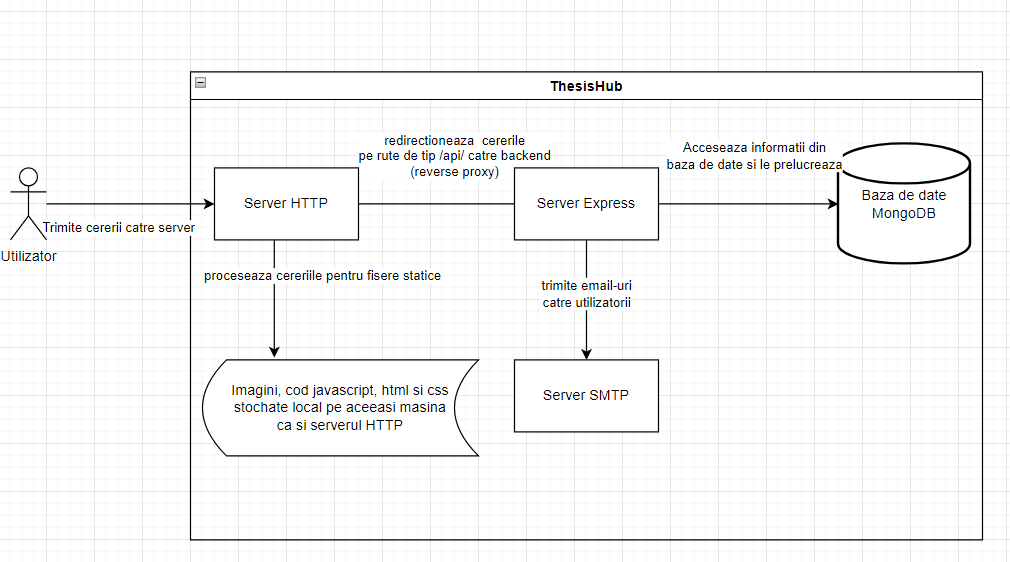
\includegraphics[scale=0.5]{images/HighLevelOverview.PNG}
    \caption{Privire de ansamblu asupra sistemului}
\end{figure}
Aplicatia poate fii impartita in urmatoarele componente:
\begin{itemize}
    \item Un server http, in momentul de fata este cel oferit de catre mediul de dezvoltare react, insa acesta poate fii inlocuit cu server http dedicat
    optimizat pentru "productie", acesta v-a reprezenta punctul de intrare in sistem, toate cererile fiind interceptate de catre el, cele pentru resurse statice 
    vor fi rezolvate de catre acesta iar cererile pe rutele de tipul /api/ vor fii redirectionate catre serverul express.
    \item Un server de tip express(backend), acesta poate fii considerat piesa centrala a aplicatiei.
    fiind cel responsabil pentru procesarea majoritatii actiunilor utilizatorilor cat si de validarea acestora si de
    obtinirea datelor necesare pentru ca clientul sa poata genera paginile dorite.
    \item Gestionarea starii este o necesitate pentru orice proiect non-trivial, iar o baza de date face acest lucru
    fezabil oferind atat persistenta datelor cat si o interfata de a lucra cu aceastea.
    \item Un server smtp, acesta permite trimiterea de email-uri de catre sistem utilizatorilor aplicatiei, email-urile reprezentand 
     in acest caz un mod de a comunica cu utilizatorii fara a fii necesara o conexiune intre cei doi.
\end{itemize}

\section{Cazuri de utilizare pentru utilizatorii standard}
\begin{figure}[h]
    \centering
    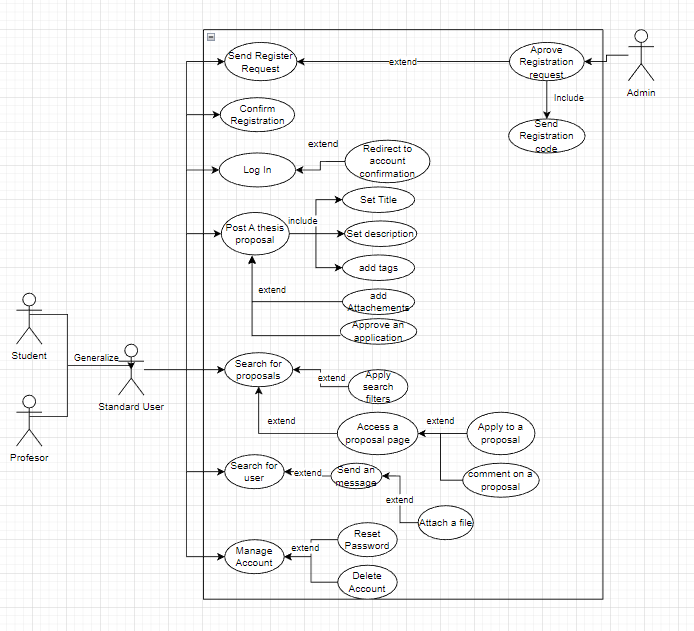
\includegraphics[scale=0.5]{images/StandardUserUseCase.png}
    \caption{Cazuri de utilizare pentru utilizatorii standard}
    \label{fig:stdUserDiagram}
\end{figure}
În diagrama de mai sus am ales să generalizez utilizatorul de tip Student și utilizatorul de tip Profesor ca un actor de tip „Utilizator standard” dat fiind faptul ca facilitățile disponibile celor  două tipuri de conturi sunt aceleași, diferențierea dintre cele două tipuri de conturi fiind totuși  necesară din punct de vedere semantic(nu ar avea sens ca aplicația să permită unui student să coordoneze lucrări, sau unui profesor să aplice pentru tema propusă de alt profesor). Am încercat să cuprind în această diagramă toate cazurile de utilizare disponibile  unui utilizator standard cu scopul de a avea o imagine generala asupra facilitaților oferite de către platforma, voi analiza detaliat însă publicarea pe platforma a unei noi propunere de lucrări:



Acest caz de utilizare descrie procesul prin care noile propuneri de lucrări sunt adăugate pe platforma
\begin{itemize}
    \item{Actorii:
        \begin{enumerate}
            \item Utilizator standard
        \end{enumerate}}
    \item{Precondi\c tii:
        \begin{enumerate}
            \item Utilizatorul este de tip Profesor sau Student
            \item Contul acestuia trebuie să fi trecut atât de aprobarea înregistrării de către un administrator al platformei cât și confirmarea acesteia de către utilizator
            \item Utilizatorul este autentificat pe platformă
        \end{enumerate}}
    \item{Scenariu:
        \begin{enumerate}
            \item Accesarea paginii pentru crearea unei propuneri de licență
            \item Introducerea unui Titlu
            \item Introducerea unei Descrierii
            \item {Selectarea etichetelor potrivite temei propuse din lista de etichete disponibile
                \begin{enumerate}
                    \item utilizatorul este nevoit să selecteze cel puțin o etichetă pentru a continua
                \end{enumerate}}
            \item Opțional: Adăugarea eventualelor Atașamente utile pentru descrierea temei propuse celorlalți utilizatorii interesați
            \item Dacă oricare dintre câmpurile menționate mai sus este invalid (gol sau prea scurt) atunci utilizatorul este avertizat
            \item Noua propunere de lucrare este creata pe platformă
        \end{enumerate}}
    \item{Postcondi\c tii:
        \begin{enumerate}
            \item Noua propunere este adăugată în baza de date a platformei și devine vizibilă celorlalți utilizatori ai platformei, ei putând interacționa cu această
        \end{enumerate}}
\end{itemize}
\section{Cazuri de utilizare pentru administratori}
\begin{figure}[H]
    \centering
    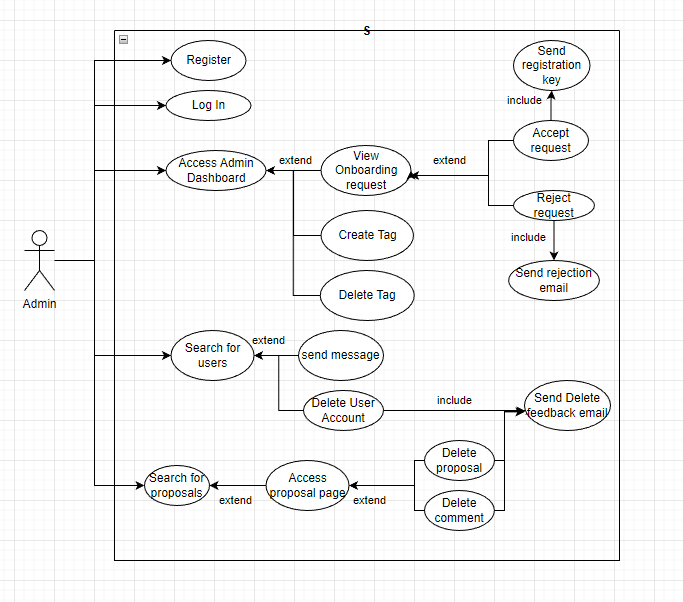
\includegraphics[scale=0.5]{images/AdminUserUseCase.png}
    \caption{Cazuri de utilizare pentru Administratori}
    \label{fig:adminUseCaseDiagram}
\end{figure}
Administratorii sunt utilizatorii cu privilegii ridicate, care au posibilitatea și responsabilitatea să gestioneze accesul celorlalți utilizatorii la platformă și să modereze conținutul acesteia pentru a păstra calitatea conținutului platformei la standardele universității și a unui mediu academic (eliminarea potențialelor postări/comentarii inadecvate scopului platformei), acest tip de conturi este gândit ca unul strict administrativ neavând astfel capacitatea de a:
\begin{itemize}
    \item Publica propuneri de lucrări.
    \item A aplica pentru propunerile existente sau de a lasă comentarii asupră acestora.
\end{itemize}
funcționalitățile comune cu conturile de utilizator standard fiind doar:
\begin{itemize}
    \item Autentificarea.
    \item Căutarea și accesarea  propunerilor de lucrări de pe platformă.
    \item Trimiterea de mesaje celorlalți utilizatori.
\end{itemize}
Am ales de asemenea că pentru diagramă de mai sus să abstractizez funcționalitatea ce ține de autentificare și trimiterea de mesaje, această fiind identică cu cea a conturilor standard reprezentate deja mai detaliat în diagrama precedentă, mai jos se poate revedea o analiză mai în detaliu a cazului de utilizare pentru aprobarea sau respingerea unei cererii de înregistrare.
\begin{itemize}
    \item {Actorii:
        \begin{enumerate}
            \item Administrator.
        \end{enumerate}}
    \item {Precond\c tii:
        \begin{enumerate}
            \item Utilizatorul are un cont de administrator pe platformă.
            \item Contul acestuia trebuie să fi trecut atât de aprobarea înregistrării de către un administrator al platformei cât și confirmarea acestuia de către utilizator.
            \item Utilizatorul este autentificat pe platformă.
            \item Există cel puțin o cerere de înregistrare pe platformă.
        \end{enumerate}}
    \item {Scenariul standard:
        \begin{enumerate}
            \item Utilizatorul accesează bordul de gestionare al administratorilor.
            \item Utilizatorul alege una dintre cererile de înregistrare.
            \item Utilizatorul verifica datele afișate în cererea de înregistrare.
            \item Utilizatorul verifica dovezile de identitate atașate de persoana care a inițiat cererea.
            \item Utilizatorul validează cererea.
            \item un email automat va fi trimis de către sistem utilizatorului care a inițiat cererea conținând un cod necesar pentru confirmarea înregistrării.    
        \end{enumerate}}
    \item {Postcondi\c tii:
        \begin{enumerate}
            \item Cererea o dată procesată va dispărea din bordul de gestionare al administratorilor.
            \item Un cod de confirmare a înregistrării este generat de către sistem și primit de către persoana care a inițiat cererea pe adresa de email folosită de către aceasta la crearea contului.
            \item Utilizatorul care a inițiat cererea are acum potențialul de își confirma contul, având apoi acces la restul funcționalităților de pe platformă.
        \end{enumerate}}
    \item {Scenariu alternativ:
        \begin{enumerate}
            \item Utilizatorul accesează bordul de gestionare al administratorilor.
            \item Utilizatorul alege una dintre cererile de înregistrare.
            \item Utilizatorul verifică datele afișate în cererea de înregistrare.
            \item Utilizatorul verifică dovezile de identitate atașate de persoana care a inițiat cererea.
            \item Utilizatorul respinge cererea.
            \item Utilizatorul este nevoit să justifice decizia de a respinge cererea.
            \item Un email de informare împreună cu justificarea respingerii oferită de către administratorul care a procesat cererea respectivă este trimis.
        \end{enumerate}}
    \item {Postcondi\c tii:
        \begin{enumerate}
            \item Cererea o dată procesată vă dispărea din bordul de gestionare al administratorilor.
            \item Contul nu a fost creat și un email de informare a fost trimis de către sistem.
        \end{enumerate}}
\end{itemize}
\section{Design-ul bazei de date}
\subsection{Privire de ansamblu}
\begin{figure}[H]
    \centering
    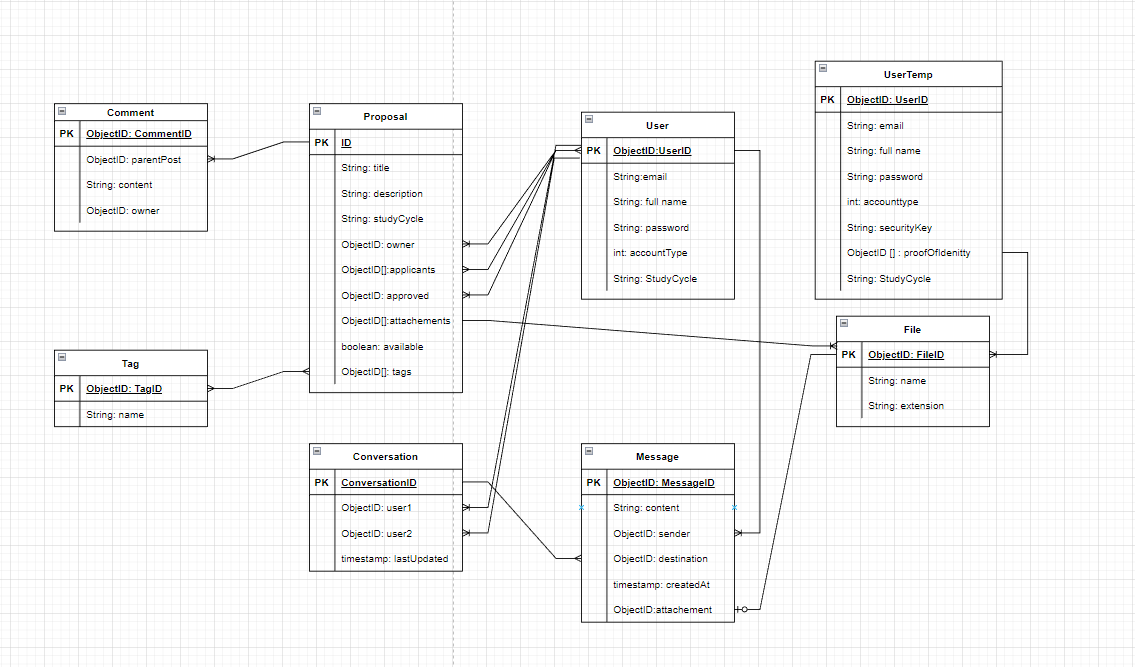
\includegraphics[scale=0.4]{images/DB_Diagram.png}
    \caption{Diagrama bazei de date}
\end{figure}
Mai jos se poate regăsii o scurta descriere a fiecărei colecții regăsite în diagrama de mai sus
\subsection{Analiza colec\c tiilor din baza de date}
\subsubsection{User}
În această colecție vor fi stocate toate documentele care conțin informații despre utilizatorii aplicației, informații precum:
\begin{itemize}
    \item Nume.
    \item Email.
    \item Parola.
    \item Tip de utilizator (Profesor, Student sau Administrator).
    \item Ciclu de studiu(Licență sau Master)    
\end{itemize}
parolele sunt de asemenea trecute printr-un algoritm de „hashing”\footnote[1]{ în acest context un proces unidirectional și determinist de a mapa un \c sir de caractere la unul nou, de lungime fixa și cu un aspect complet aleatoriu pentru un eventual actor malițios care a obținut acces la baza de date} înainte de a fi stocate din motive de securitate.
\subsubsection{UserTemp}
În această colecție sunt stocate cererile de înregistrare pe platformă, pe lângă câmpurile din colecția „User” avem un câmp în plus care va stoca o cheie de confirmare și referințe către dovezile de identitate aferente cererii din colecția de fișiere, în momentul când utilizatorul creează o cerere de înregistrare pe platformă un document nou va fi creat în această colecție având câmpul cheii de confirmare nul, o dată validată cererea de către administrator o cheie de confirmare va fi generată pentru acest utilizator și transmisă acestuia prin email, odată cu confirmarea înregistrării de către utilizator folosind cheia primită un document nou va fi creat în colecția "User" iar cel aferent cererii de înregistrare va fi șters din colecția „UserTemp”.
\subsubsection{Comment}
În această colecție sunt stocate comentariile de pe platformă, pe lângă conținutul comentariului se mai stochează și o refererin\c ta către utilizatorul care a postat comentariul și către propunerea de tema asupra căreia a fost lăsat comentariul.
\subsubsection{Tag}
În aceasta colecție se găsesc etichetele pe care un utilizator le poate atașa unei propuneri la creare, ștergerea și adăugarea de documente noi în aceasta colecție este rezervată exclusiv administratorilor
\subsubsection{Conversation}
Această colecție servește funcționalita\c tii de mesagerie a platformei, aici sunt stocate conversațiile (doar membrii, nu și conținutul) de pe platformă, împreuna cu o data care reprezintă data și timpul ultimului mesaj nou în aceea conversație(necesar pentru afișarea conversațiilor unui utilizator în ordine cronologică.
\subsubsection{Message}
Această colecție stochează mesajele trimise de către utilizatorii, atributul „sender” conține id-ul utilizatorului care a trimis mesajul iar cel de „destination„ conține id-ul conversației în care a fost trimisă, utilizatorul   care dorește să trimită un mesaj nou trebuie evident să fie un membru al acelei conversații.
\subsubsection{File}
Această colecție stochează numele fișierelor aferente platformei și extensia acestora, fișierele în sine fiind stocate în sistemul de fișiere al serverului, această colecție stocând doar referințe către acestea.
\subsubsection{Proposal}
această colecție stochează propunerile de teme de pe platformă, aceasta deține câmpuri primitive precum:
\begin{itemize}
    \item Descriere.
    \item Titlu.
    \item Ciclu de studiu.
    \item Disponibilitate.
\end{itemize}
dar și referințe către alte colecții precum:
\begin{itemize}
    \item "owner” reprezintă id-ul utilizatorului care a publicat propunerea de tema.
    \item „applicants” reprezintă un vector de id-uri ale unor utilizatori care au aplicat pentru propunerea în cauză.
    \item „attachaments” un vector de id-uri către fișierele aferente propunerii.
    \item „tags” conține referințe către etichetele atașate propunerii.
    \item „approved” conține o referința către utilizatorul a cărui aplicație a fost aprobată de către „owner” această referința este nula la creare și rămâne așa până când o aplicație este aprobată.
\end{itemize}
\chapter{Detalii de implementare}
\section{Tehnologiile alese}
\subsection{Frontend}
\subsubsection{Javascript}
Javascript\cite{5} este un limbaj de programare interpretat conceput inițial pentru a rula în browser cu scopul de a
manipula conținutul paginilor web și de a facilita astfel aplicații web cu conținut dinamic.

Acesta este un limbaj de programare de nivel înalt, oferind facilități precum : tipizare dinamica, gestionare automată
a memoriei și suport atât pentru programare funcționala, tratând funcțiile ca obiecte de ordin prim,
cât și pentru programarea orientată pe obiecte. În plus Javascript dispune de o bibliotecă standard vastă care să acopere
majoritatea nevoilor dezvoltatorilor cu privire la funcționalități "low level", atât expresivitatea limbajului
cât și timpul relativ scurt de învățare a acestuia au contribuit la creșterea popularității sale.

În momentul de fața Javascript se regăsește ca unul dintre cele mai folosite limbaje de programare,
acesta fiind între timp extins în afara limitelor unui browser datorita tehnologiilor precum React Native și NodeJS;

\subsubsection{React}
React\cite{1} este un framework pentru dezvoltarea interfețelor web
care are la bază conceptul unui DOM virtual care să servească ca o interfața/intermediar a DOM-ului browser-ului,
Acest DOM virtual este reprezentat nativ în Javascript și stochat în memoria sistemului client, făcând astfel
manipularea acestui DOM virtual de către Javascript mult mai puțin costisitoare.

Un alt concept fundamental pentru react sunt componentele, acestea stând la baza oricărui proiect react.
Componentele au în definiția lor atât o reprezentare în DOM-ul virtual cât și stare, starea în acest context
poate fi interpretată ca și elementele non-statice dintr-o pagină web, care depind de utilizator și acțiunile sale.
odată ce starea unei componente a fost modificată este inițiat un proces de reconciliere între  DOM-ul virtual și DOM-ul
browser-ului în urma căruia doar părțile care diferă dintre cele două DOM-uri sunt rerandate în pagina web, celelalte părți 
rămânând intacte. Datorită acestui fapt aplicațiile react tind să ofere o experiență de utilizare fluidă în schimbul
unui consum de memorie crescut.

Componentele de tip react pot conține în definiția lor atât componente primitive cât
și alte componente compuse iar componentele pot împărtăși în mod selectiv parți din starea lor cu componentele
din care sunt compuse, în acest fel, componentele care depind de stare comună între ele nu sunt nevoite să
gestioneze această stare în paralel, ci, în mod uzual starea comună împreună cu responsabilitatea gestionării ei 
este elevată la cel mai apropriat părinte comun al acestora iar starea este transmisă mai apoi în cascadă spre componentele care depind de ea. 

Atât procesul simplu de gestionare a stării cât și
posibilitatea de îmbricare a componentelor duc spre două principii fundamentale în filosofia react,
mai exact compozabilitate și reutilizabilitate, aceste 2 principii dovedindu-se extrem de utile în gestionarea complexități.
Rata de adopție a react-ului a fost una foarte abruptă datorită funcționalităților inovative pentru timpul lor pe care le-a adus acesta
fiind în momentul de față de departe cel mai popular frontend framework.

\subsubsection{CSS}

CSS (Cascading Style Sheets) este un limbaj pentru descrierea stilului paginilor web. Deși HTML-ul permite stilizarea elementelor individuale folosind atributul de stil (Inline Styling) 
această abordare devine ineficientă în cazul unui proiect de complexitate ridicată. În mod uzual, HTML-ul este utilizat pentru a defini doar scheletul paginii web, 
în timp ce aspectul paginii este delegat CSS-ului. 

CSS oferă funcționalități precum moștenirea stilurilor, posibilitatea de a grupa elementele, aplicarea de stiluri pe grupuri de elemente și un sistem intuitiv de rezolvare a conflictelor. 

Apariția CSS a reprezentat un pas uriaș în evoluția dezvoltării web, revoluționând practic acest domeniu. Deși există alternative precum Sass, 
Less și Stylus, acestea sunt, în esență, doar extensii ale CSS-ului, iar codul scris în aceste limbaje este compilat în CSS înainte de a fi procesat de către browser. 
CSS nu are, astfel, vreun competitor real în această perspectivă

\subsection{Backend}
\subsubsection{NodeJS}
NodeJS\cite{3} este un mediu de rulare dezvoltat pentru a permite execuția programelor scrise în Javascript direct de către sistemul de operare, acesta a fost dezvoltat cu asincronicitate ca o prioritate,
in special pentru operațiile de Intrare/Ieșire de date (I/O) ele fiind principala motivație pentru dezvoltarea acestei tehnologii.

Creatorul nodeJS era nemulțumit de abordarea clasică din aceea perioadă de a gestiona operațiile de Intrare/Ieșire pe serverele web, mai exact abordarea în care pentru fiecare cerere primită un nou fir de execuție era creat, 
această abordare este ineficientă deoarece acele fire de execuție sunt blocate până la finalizarea operației I/O,
consumând totuși  resurse între timp(memoria rezervată firului de execuție și timpul de procesare folosit pe schimbarea de context). 

NodeJS a fost proiectat în schimb să ruleze pe un singur fir de execuție
având la baza o buclă de evenimente, interpretorul de Javascript trece prin fiecare linie de cod și când acesta întâmpină cod asincron, precum citirea dintr-o bază de date, delegă operațiile în cauza sistemului de operare.

Bucla de evenimente rulează continuu și verifică dacă operațiile delegate sistemului de operare și-au terminat execuția, în caz afirmativ aceasta apelează o funcție definită să ruleze odată cu finalul execuției codului asincron aferent
(Callback function), Arhitectura NodeJS-ului este principalul motiv datorita căruia acesta este recunoscut și apreciat pentru scalabilitatea sa. 

Deși o tehnologie relativ recentă, aceasta a avut o creștere în popularitate
remarcabilă, fiind astăzi unul dintre cele mai populare tehnologii pentru backend, atât popularitatea deja existentă a Javascript-ului cât și ușurința de a îl învață, împreună cu 
conveniența de a folosi un singur limbaj de programare atât pe backend cât și pe frontend sunt principalele cauze ale popularității sale, coborând de astfel considerabil
bariera de intrare pentru dezvoltarea web, fiind un favorit pentru începătorii din acest domeniu.
\subsubsection{Express}
Express\cite{2} este un framework minimalist și neopinionat al nodeJS-ului dedicat pentru dezvoltarea serverelor web, acesta poate fi considerat minimalist deoarece oferă
o suită relativ mică de facilități, focusându-se pe anumite funcționalități generale, de exemplu: rutarea cererilor http, ușurând procesul de a lucra cu rute dinamice și oferind posibilitatea de a grupa rutele, un sistem
de gestiune a fluxului cerere-răspuns, și suport pentru șablonarea paginilor în cazul aplicațiilor unde randarea se face pe server.

Express prioritizează integrabilitatea și extensibilitatea să cu alte librării, delegând comunității datoria de a dezvolta librării pentru a acoperii cazuri de utilizare specifice și dezvoltatorului datoria de a se documenta și alege "uneltele" necesare pentru proiectul său.

Acesta mai este descris și ca neopinionat deoarece își propune să nu impună dezvoltatorilor o anumită paradigmă, arhitectura software
sau set de convenții / "bune practici" lăsând dezvoltatorilor atât libertatea cât și responsabilitatea de a alege acestea în funcție de particularitățile proiectului și a echipei în care lucrează. 

Abordarea liberală a expressului a rezultat într-un ecosistem vast și în continua creștere în jurul sau, fiind astăzi unul dintre cele mai populare librarii NodeJS folosite.

O funcționalitate care stă la baza express-ului este support-ul pentru middleware, pentru fiecare ruta definită avem cel puțin o funcție care va fi apelata odată cu intrarea
unui cererii pe aceea ruta,
important este însă faptul ca express ne permite să adăugăm și o lista de funcții intermediare care vor fi apelate secvențial, oricare dintre acestea putând oprii prematur execuția(de regula în cazuri de eroare) 
sau de a apela următoarea funcție din lanț, opțional acestea pot și adăuga/modifica date din cererea primită înainte de a apela următoare funcție, 
acesta reprezentând un mecanism de a persista stare între diferitele funcții implicate în ciclul de viață al unei cererii, acest fapt crescând semnificativ potențiala modularitatea a codului
\subsubsection{MongoDB}
MongoDB\cite{4} este un sistem de gestionare a bazelor de date de tip NoSQL bazat pe documente
(echivalentul rândurilor într-o baza de date de tip SQL) și colecții (echivalentul tabelelor în baze de date SQL), 
documentele sunt scrise în format BSON (Binary Javascript Object Notation), 
Acest format suportând obiecte(imbricarea obiectelor fiind suportată de asemenea) și vectorii 
de valorii primitive sau de obiecte în plus fata de tipurile primitive comune cu SQL, 
Acest fapt oferă o flexibilitate semnificativ mai mare în proiectarea 
unei baze de date spre deosebire de un DMBS de tip SQL, 
această flexibilitate vine însă la costul consistenței, o colecție nu impune 
în mod nativ o schemă asupră documentelor pe care le are în apartenentă, 
astfel în mod teoretic se poate ca două documente din aceiași colecție să aibă o structura diferita, 
de regulă sunt impuse însă soluții de validare a operațiunilor de creare/modificare 
pentru a putea asigura o consecvența a datelor.
\subsubsection{Mongoose}
Mongoose este o librărie de mapare a datelor în obiecte (Object-Data Modeling), ODM-urile 
oferă o interfață de tip OOP în limbajul de programare ales pentru a interacționa cu baza de date NoSQL aleasa,
condiția fiind evident ca ODM-ul ales să suporte atât
limbajul de programare ales cât și baza de date. Mongoose oferă o interfață în javascript pentru 
a interacționa cu baze de date de tip MongoDB, pe lângă aceasta conveniența de a putea comunica cu baza de date 
scriind cod direct în javascript și suita de funcții care abstractizează detalii de implementare ale unor
nevoi comune(de exemplu findByIdAndDelete), acesta mai are un beneficiu foarte important  
deoarece ajuta în diminuarea principalului dezavantaj al MongoDB-ului, mai exact lipsa de consistență.
Mongoose interacționează doar cu colecțiile din baza de date pentru care are un model definit, la baza acestui 
model stă o schema definită în JSON pe care obiectele din aceea colecție ar trebui să o respecte. Orice încercare
de a crea / modifica obiecte în așa fel încât nu vor respecta schema definită va genera o eroare, acest lucru 
nu rezolva în totalitate problema din păcate însă deoarece validează doar operațiile de scriere pe care acesta le primește,  
baza de date putând fi încă modificata direct și astfel aceasta ar putea ajunge într-o stare inconsistentă. 
Practic mongoose garantează consistența bazei de date doar dacă scrierea în aceasta se face în mod exclusiv
prin mongoose.
\subsection{General}
\subsubsection{HTTP}
HTTP(Hypertext Transfer Protocol) este un protocol de comunicare construit pe baza protocolului TCP/IP cu scopul de a standardiza
comunicarea între clienți și serverele web, acesta urmează modelul "cerere-răspuns", în care
clientul și server-ul stabliesc o conexiune, clientul apoi trimite o cerere serverului iar serverul trimite înapoi un răspuns,
după care conexiunea este închisă, protocolul HTTP stă la baza web-ului acesta fiind protocolul folosit pentru marea majoritate
a traficului web, acesta are o limitare însă, cum conexiunea poate fi inițiată doar de către client, iar aceasta este închisă automat odată cu
primirea răspunsului din partea serverului cererile de tip HTTP nu sunt potrivite pentru cazurile de utilizare unde se dorește ca serverul să 
trimită mesaje către client, cum ar fi în cazul de față funcționalitatea pentru mesagerie, în care se dorește ca serverul 
să trimită clientului mesajele primite în timp real. Exista câteva "soluții" pentru a suporta această funcționalitate, cum ar fi HTTP polling
unde clientul trimite cereri către server pentru a obține mesajele noi la un interval fix de timp, problema cu această abordare fiind
echilibrul dintre responsivitate și performanță, în această abordare dacă timpul de așteptare dintre cereri este prea lung atunci experiența utilizatorului
se degradează considerabil, însă dacă cererile sunt prea frecvente atunci performanța sistemului va avea de suferit, crescând drastic numărul de cereri
trimise în timp ce majoritatea acestora vor fi redundante.

O altă soluție ar fi HTTP long polling, unde se trimite o singură cerere, iar serverul blochează acel fir de execuție(fiind creat un fir de execuție diferit pentru fiecare cerere) până când
acesta are date de trimis clientului, după care răspunsul este trimis și conexiunea este închisă, iar apoi clientul inițiază o nouă astfel de cerere,
aceasta abordare este mai eficienta decât prima însă este tot suboptima, deoarece o buna parte din resursele serverului vor fi blocate la orice moment dat.
\subsubsection{WebSockets}
WebSockets este un protocol construit cu scopul de a rezolva problemele cauzate de limitările protocolului HTTP, construit tot pe baza TCP/IP acesta oferă 
posibilitatea unei comunicări bidirecționale și cu latență redusa între client și server, făcând astfel aplicațiile web care necesită comunicare în timp real
fezabile, în acest protocol conexiunea dintre client și server este proiectată să persiste iar atât clientul cât și serverul pot să trimită evenimente
celuilalt oricând iar aceste mesaje sunt mult mai rapide deoarece acestea nu trebuie să includă "bagajul" necesar pentru stabilirea unei conexiuni noi 
spre deosebire de http
\section{Manual de Implementare}
\subsection{Backend}
\subsubsection{Arhitectura sistemului}
fișierele care conțin codul sursă sunt împărțite logic în următoarele categorii:
    \begin{itemize}
        \item {
            Models: acest folder conține modelele mongoose aferente colecțiilor din baza de date
        }
        \item {
            Controller: în acest folder se regăsesc funcțiile definite pentru a trata cererile primite
        }
        \item{
            Routes: aici sunt definite rutele pe care le accepta serverul și sunt legate de funcțiile care ar trebui să ruleze la apelarea rutelor respective
        }
    \end{itemize}
    după cum se poate observa în figura 4.1 există o mapare de aproape 1:1 între modele și controllere,
    arhitectura implementată a fost în mare parte inspirată de către MVC(Model View Controller), funcțiile care creează/returnează/modifică sau șterg
    obiecte ce aparțin de un anumit model sunt grupate sub un singur fișier numit controller legat logic de model-ul aferent, această implementare
    nu respectă în totalitate arhitectura MVC totuși , deoarece backend-ul în acest caz este un rest api care comunică în mod exclusiv prin JSON
    fișierele statice(HTML, CSS și javascript) nefiind sub responsabilitatea acestuia, partea de View lipsind astfel complet din această arhitectură.
    \begin{itemize}
        \item Config: aici se regăsesc funcții pentru conectarea la baza de date 
        și conectarea serverului de express cu serverul de SMTP pentru funcționalitățile ce implică trimiterea de email-uri
        \item Middleware: acest folder conține funcțiile intermediare rulate înainte de cele din controller, în mare parte funcționalitate pentru validarea request-ului
        dar sunt și unele funcții menite pentru a adăuga informații în request-ul primit de la client
        \item Utils: aici se regăsește de regulă cod necesar/util care nu potrivește însă nici unei alte locații din punct de vedere semantic.
        în cazul de față o clasa care extinde clasa de baza "Error", care primește ca și attribut pe lângă un mesaj de eroare și un cod de status
        util în generarea și tratarea erorilor întâmpinate de un server web
    \end{itemize}
    \subsubsection{fluxul de control}
    Pentru a putea înțelege mai bine modul de funcționare a serverului, consider că ar fi utilă urmărirea cap-coadă a ciclului de viață a unui request, 
    în cazul de față o cerere care constă în aprobarea unei aplicații ar fi ceea mai potrivită.
    
    Odată cu pornirea serverului, acesta creează o instanță nouă de express, și îi specifică acesteia că pentru oricare cerere a cărei 
    destinații începe cu "api/proposal" să folosească rutele definite în proposalRoutes.
    \begin{lstlisting}[language=Javascript]
        import express from "express";
        import proposalRoutes from "./routes/proposalRoutes.js";

        const app = express();
        app.use("/api/proposal", proposalRoutes);
    \end{lstlisting}
    în acest set de rute o avem pe următoarea definită: "/:proposalID/approve" unde ":proposalID" este un parametru, acesta nu are o valoare predefinită,
    ci este mai degrabă un substituent, practic orice request de tipul: /api/proposal/<id>/approve  
    unde id poate să ia orice valoare va intra pe această rută, valoarea acestuia fiind făcută disponibilă funcțiilor care
    tratează cererea, acestea putând accesa proprietatea req.params.proposalID
    \begin{lstlisting}[language=Javascript]
        import express from "express";
        import { auth } from "../middleware/auth.js";
        import {addProposalToReq,
            isProposalOwner,
            validateApproval} from "../middleware/validators/proposalValidator.js";
        import {approveApplication} from "../Controllers/proposalController.js";
        import { isAuthorized } from "../middleware/validators/userValidator.js";

        const router = express.Router();
        router.put("/:proposalID/approve", auth,
            addProposalToReq,
            isProposalOwner,
            isAuthorized,
            validateApproval,
            approveApplication);
        export default router;
    \end{lstlisting}
    Odată intrat un astfel de request, prima funcție care se apelează este ce de autorizare,
    pentru a vorbi despre aceasta însă, consider că o scurtă explicație despre Json Web tokens (JWT)
    este necesară deoarece aceasta tehnologie stă la baza sistemului de autentificare și autorizare.
    
    în urma unei autentificări reușite
    serverul generează un hash pe baza încărcăturii token-ului (payload-ul, în cazul de față id, tip cont și ciclu de studii)
    timpul și o cheie secretă data serverului ca și variabila de mediu (environment variable), token-ul nu poate fi descifrat
    fără a avea acces la cheia secretă  folosită pentru a genera hash-ul iar token-ul nu poate fi alterat de  către 
    un eventual actor malițios deoarece oricare alterare va rezulta într-un hash invalid
    (modificarea unui singur caracter oarecare din cele folosite pentru generarea token-ului va genera un hash complet diferit, astfel
    nu se poate "ghici" ce modificare pot fi aduse unui token deja existent pentru a îi modifica payload-ul), Odată acest token primit
    clientul îl salvează în memoria locală și îl atașează la fiecare request, serverul cunoscând secretul cu care a fost "semnat" token-ul
    îl poate descifra pentru a avea acces la acest payload și astfel identifica cine este utilizatorul care a inițiat request-ul în cauză.
    Revenind la funcția noastră, aceasta verifică dacă requet-ul primit conține un header de autorizare de tip "Bearer token",
    și dacă da, încearcă să îl descifreze folosind codul secret, în cazul în care header-ul este prezent și poate fi descifrat (este valid) atunci
    adaugă în request payload-ul token-ului și apelează următoarea funcție din lanț, în caz contrar trimite clientului un răspuns de tip eroare și oprește procesarea acelui request
    \begin{lstlisting}[language=Javascript]
        import jwt from "jsonwebtoken"

        function auth (req, res, next){
            if(req.headers.authorization &&
            req.headers.authorization.startsWith("Bearer")){
                try {
                    let token = req.
                     headers.
                     authorization
                     .split(" ")[1];
                    req.user = jwt
                     .verify(token, process.env.AUTH_SECRET);
                    next();
                } catch (error) {
                    console.log(error)
                    return res.status(500).json(error);
                }
            }
            else{
                return res.
                 status(400)
                 .json({msg:"auth token not found or invalid"})
            }
        }
    \end{lstlisting}
    următorul pas este să verificăm dacă id-ul primit ca și parametru este unul valid, mai întâi verificăm dacă s-a primit o valoare pentru acest ID sau acesta este null
    iar în caz afirmativ, obținem din baza de date obiectul aferent acelui ID și îl atașăm cererii în același mod ca și în pasul anterior 
    iar într-un final apelăm următoarea funcție din lanț. în cazul însă în care nu a fost oferit un ID sau nu există acest ID în baza de date, returnăm din nou eroare
    \begin{lstlisting}[language=Javascript]
    async function addProposalToReq(req, res, next){
        try {
            validateString(req.params.proposalID);
            const proposal = await Proposal
                .findById(req.params.proposalID)
                .populate({
                    path: "owner",
                    model: "User"
            })
            if(!proposal){
                throw new customError(```the proposal ID provided
                 does not exist```, 400);
            }
            req.post = proposal;
            next();
        } catch (error) {
            if(error instanceof customError){
                return res
                 .status(error.statusCode)
                 .json({msg: error.message})
            }
            console.log(error);
            return res.status(500).json(error);   
        }
}
    \end{lstlisting}
    următorul pas este să verificăm dacă utilizatorul care a inițiat cererea este și destinatorul propunerii de teme,
    în caz afirmativ, se adaugă un nou atribut în request, numit auth și este setat ca adevărat.
    La final se apelează următoarea funcție din lanț indiferent de rezultatul condiției
    \begin{lstlisting}[language=Javascript]
        async function isProposalOwner (req, res, next){
        try {
            if(req.user.id == req.post.owner._id){
                req.auth = true;
            }
            next();
        } catch (error) {
            return res.status(500).json({msg: error});
        }
    \end{lstlisting}
    apoi se verifică dacă utilizatorul este autorizat sau nu pentru a iniția cererea în cauză, acest lucru se face verificând
    dacă vreo funcție anterioară lui "isAuthorized" a setat deja atributul "req.auth" ca adevărat, în caz afirmativ
    acesta apelează doar funcția următoare din lanț, iar în caz contrar returnează o eroare de tipul "permisiuni insuficiente"
    această abordare simplifică semnificativ implementarea unui sistem de permisiuni complex, dat fiind modularitatea sa
    acesta presupune doar definirea unor middleware-uri care verifică unele condiții simple, și apoi la definirea rutei
    acestea se pot înlănțui în funcție de nevoie, un exemplu pentru asta ar putea fi: o rută pentru ștergerea unui comentariu
    și o rută pentru editarea unui comentariu, ar avea sens ca atât persoana care a postat comentariul, 
    cât și persoana care deține postarea în care a fost postat comentariul, cât și un administrator să poată șterge comentariul în cauză 
    însă doar persoana care a postat comentariul ar trebui să aibă permisiunea de a îi modifica conținutul, în acest context
    ambele cazuri se pot rezolva implementând următoarele funcții: isCommentOwner, isProposalOwner, isAdmin în același mod ca și în pasul precedent
    iar apoi pentru ruta de ștergere apelăm următoarea listă de funcții "..., isCommentOwner, isProposalOwner, isAdmin, isAuthorized, ..."
    iar pentru cea de editare apelăm doar "...,isCommentOwner, isAuthorized, ..."
    \begin{lstlisting}[language=Javascript]
        async function isAuthorized(req, res, next){
        try {
            if(!req.auth)
                return res
                 .status(400)
                 .json({msg: ```Insufficient permissions
                 to proceed with this request```});
            next();
        } catch (error) {
            console.log(error);
            return res.status(500).json({msg: error});
            
        }
    }
    \end{lstlisting}
    după autorizare, următorul pas este validarea cererii, funcția verifică dacă propunerea respectivă are deja o aplicație aprobată
    și dacă id-ul utilizatorului aplicant lipsește din baza de date, dacă cel puțin una dintre aceste două sunt adevărate atunci funcția va returna o eroare și va opri execuția
    în caz contrar, se apelează ultima funcție din acest lanț
    \begin{lstlisting}[language=Javascript]
        async function validateApproval(req, res, next){
        try {
            if(req.post.approved){
                throw new customError(```you have already approved
                 an application for this particular proposal```, 400);
            }
            const user = await User
            .findById(req.body.applicantID);
            if(!user){
                throw new customError(```the provided applicant ID
                 does not exist```, 400);
            }
            next();
        } catch (error) {
            if(error instanceof customError){
                return res
                .status(error.statusCode)
                .json({msg: error.message})
            }
            console.log(error);
            return res.status(500).json(error);   
        }
    }
    \end{lstlisting}
    pasul final, atributul "approved" al postării este modificat din null în id-ul utilizatorului a cărui aplicație a fost aprobată
    și apoi funcția trimite un răspuns cu un mesaj de succes clientului
    \begin{lstlisting}[language=Javascript]
        async function approveApplication (req, res){
        try {
            const post = req.post;
            post.approved = req.body.applicantID;
            await post.save()
            return res
             .status(200)
             .json({msg: "application approved!"});
        } catch (error) {
            console.log(error);
            return res.status(500).json(error);
        }
}
    \end{lstlisting}
\subsection{frontend}
\subsubsection{arhitectura sistemului}
Codul sursa este împărțit în următoarele categorii:
\begin{itemize}
    \item Pages: aici se regăsesc componentele React aferente paginilor platformei,
    acestea sunt componentele la cel mai înalt nivel de abstractizare, fiind compuse la rândul lor
    din alte componente React de nivel înalt.
    \item css: în acest folder se regăsesc toate fișierele ce țin de stilizarea componentelor, codul sursă de css
    a fost împărțit în fișiere în funcție de pagina de care aparține
    \item api: Acest folder conține funcțiile folosite pentru trimiterea de cereri http către backend, funcțiile respective sunt importate în anumite componente React 
    și apelate în urma unor evenimente(de exemplu la încărcarea inițială a componentei sau în urma unei apăsări de buton de către utilizator). 
    Comunicarea cu server-ul pentru funcționalitatea de mesagerie nu se regăsește aici însă, pentru această componentă comunicarea cu serverul este realizată folosind protocolul 
    WebSockets și nu http, evenimentele după care client-ul "asculta" pot fi definite doar după stabilirea unei conexiuni cu clientul, din acest motiv
    logica ce ține de mesagerie a fost încapsulată în pagina dedicată pentru mesagerie.
    \item Images: Aici se regăsesc imaginile ce țin de aplicația web în sine, acest folder este diferit de cel ce conține 
    atașamentele aferente mesajelor/propunerilor de pe platformă. În cazul de față acest folder conține logo-ul aplicației
    \item Utils: în acest folder se regăsește funcționalitatea de validare de pe front, aceste funcții sunt apelate înainte de trimiterea unor cereri către server. 
    Este de preferat identificarea cererilor greșite preventiv pe cât de mult posibil, deoarece dacă suntem într-o situație în care putem ști sigur că cererea va rezulta într-o eroare încă de pe front-end(un câmp obligatoriu lipsește de exemplu), 
    atunci clientul poate să îl anunțe pe utilizator direct, evitând astfel trimiterea unei cereri și așteptarea unui răspuns pentru ea.
    reducând în acest fel atât timpul de așteptare al utilizatorului cât și încărcătura pe care o suportă server-ul
    \item Components: în acest fișier sunt grupate restul componentelor de tip React.
    Aici se regăsesc atât componente simple (a căror definiții dețin doar elemente primitive) cât și componente de nivel înalt 
    (a căror definiție conțin alte componente de tip React). 
    Pentru a exemplifica diferența dintre cele două tipuri putem compara două astfel de componente, cum ar fi Checkbox și taglist:
    după cum se poate observa mai jos componenta Checkbox este compusă dintr-un div(container) și un element de tip p (paragraf)
    ambele putând fi considerate elemente primitive.
    \begin{lstlisting}[language=Javascript]
    export const Checkbox = ({text,
     tagID,
     checked,
     onClick}) => {
        function handleChange(){
            onClick({tagID, text});
        }

        return(
            <div className = {checked ?
            "checkbox-checked"
            :"checkbox-unchecked"}
            onClick={handleChange}>
                <p>{text}</p>
            </div>
        )
    }
    \end{lstlisting}
    Componenta TagList însă are în definiția sa alte componente compuse de tip React după cum se poate vedea, 
    din acest motiv poate fi considerată ca o componentă de nivel înalt
    \begin{lstlisting}[language=Javascript]
    export const TagList = ({tags,
     onChange,
     resetView,
     resetTags,
     categoryID})=>{
        return (
            <div className="taglist">
                <button onClick={resetView}
                className="checkbox-unchecked">
                    back to categories
                </button>
                <button onClick={resetTags}
                className="checkbox-unchecked">
                    reset tags
                </button>
                <Divider orientation='horizontal' />
                <div className="taglist-tags">
                {
                    tags.map(tag =>{
                        return (tag.category == categoryID)?
                        <Checkbox text={tag.text}
                            tagID = {tag.id}
                            checked = {tag.checked}
                            onClick = {onChange}
                            key = {tag.id} >
                        </Checkbox> : null;
                    }) 
                }
                </div>
            </div>
        )
}
    \end{lstlisting}
\end{itemize}
\subsubsection{Ierarhia componentelor}
prima componentaă din ierarhie este App, aceasta incorporează de fapt întreaga aplicație, react-ul generează "aplicații cu o singură pagină" (Single Page Applications),
mai exact la accesarea pagini se trimite către client codul necesar pentru a putea genera întreaga aplicație, în mod clasic clientul
face o cerere spre server și primește codul html, css și javascript pentru fiecare navigare între pagini, fiecare pagină fiind separată, React însă
doar manipulează dom-ul browser-ului pentru a randa subcomponente diferite a acestui element de rădăcina în funcție de URL pe care se află utilizatorul și simulând 
astfel comportamentul unei aplicații cu mai multe pagini
\begin{lstlisting}[language=Javascript]
    import { AuthPage } from './Pages/AuthPage';
    import { HomePage } from './Pages/HomePage';
    import { CreateProposalPage } from './Pages/CreateProposalPage';
    import { ProposalPage } from './Pages/ProposalPage';
    import { MessagesPage } from './Pages/MessagesPage';
    import { AdminDashboard } from './Pages/AdminDashboard'

    function App() {
    return (
        <Router>
            <Routes>
            <Route path='/' element={<HomePage/>}/>
            <Route path='/auth' element={<AuthPage/>}/>
            <Route path='/proposal/create'
             element = {<CreateProposalPage/>}/>
            <Route path='/proposal/:proposalID'
             element ={<ProposalPage/>}/>
            <Route path="/messages/"
             element = {<MessagesPage/>}/>
            <Route path="/admin/"
             element = {<AdminDashboard/>}/>
            </Routes>
        </Router>
    )
}
export default App;   
\end{lstlisting}
În cazul de față pentru fiecare rută definită este asociată o componentă de tip pagină.
Una dintre ele este pagina propunerilor, aceasta este o rută dinamică, id-ul propunerii fiind dat ca parametru.
Această pagină are în componența sa:
\begin{itemize}
    \item Bara de navigare: aceasta componenta conține butoane pentru redirectarea spre celalalte pagini și este regasita dealtfel în toate celelalte pagini
    \item ProposalItem: aceasta componenta conține datele propunerii, mai exact: titlu, descriere, detinator, ciclu de studii, etichete(tags) și atașamentele propunerii
    \item CommentSection: aceasta componenta conține atât lista de comentarii de pe platforma cât și componenta pentru adăugarea comentariilor noi
\end{itemize}
\begin{lstlisting}[language=Javascript]
    <div className="ProposalPage">
        <Navbar/>
        <VStack>
            <div className="proposal-page-main-main">
                {!loading && <ProposalItem 
                    proposalData={proposal} 
                    updateProposalApplications = {updateProposalApplications} 
                    updateProposalApproved = {updateProposalApproved}/>}
                <CommentSection proposalID={proposalID}/>
            </div>
        </VStack>
    </div> 
\end{lstlisting}
componenta "Comment-section" primește de la părinte id-ul cererii, și la înaintarea acesteia
trimite o cerere spre server pentru a obține lista de comentarii aferente propunerii, iterează 
apoi prin lista primită și generează un CommentItem(comentariu) pentru fiecare element din listă.
\begin{lstlisting}[language=Javascript]
    {
    !isloading &&
    <div className="Comment-section">
        <div className="Comments" ref={commentListRef}>
            {
                commentList.map(comment =>{
                    return <CommentItem 
                     key={comment._id} 
                     comment={comment}/>
                })
            }
        </div>
        <div className="Add-comment">
            <textarea id="message" 
             name="message" 
             placeholder= {`press <Shift> + <Enter>
              to send the message ...`}
             ref={textboxRef} 
             onKeyDown={(e)=>{handleChange(e)}}>
            </textarea>
        </div>
    </div>
    }
\end{lstlisting}
Iar componenta "comment-item" primește de la componenta părinte conținutul comentariului ca și stare
și pe baza acestuia se generează conținutul comentariului, sintaxa JSX permite definirea de blocuri de cod javascript(intre acoloade)
aceste blocuri permit să generăm conținut dinamic, componentele putând astfel avea variabile în definițiile lor.
Această sintaxă ne permite și să randăm în mod condițional un element, după cum se poate vedea mai jos, 
iconița aferentă autorului comentariului este definită condițional folosind operatorul terțiar în funcție de tipul de cont 
al autorului.
\begin{lstlisting}[language=Javascript]
import { GiTeacher } from "react-icons/gi";
import { FaUserGraduate } from "react-icons/fa";
export const CommentItem = ({comment}) =>{
    return(
        <div className="comment-item">
            <p>{comment.content}</p>
            <div className="comment-item-footer">
                <div className=
                 "comment-item-footer-nameAndType">
                    {comment.owner.type === "Student" ?
                     <FaUserGraduate/>:
                     <GiTeacher/>}
                    <p>{comment.owner.name}</p>
                </div>
                <p>{new Date(comment.postedAt)
                 .toLocaleDateString("ro-RO", 
                 { 
                    day: "numeric",
                    month: "numeric",
                    year: "numeric"
                 })
                }</p>
            </div>
        </div>
    )
}
\end{lstlisting}
\section{manual de utilizare}
Primul pas necesar pentru a putea folosi platforma este trimiterea unei cereri de înregistrare, pentru asta este necesar
ca utilizatorul să acceseze formularul de înregistrare și să completeze următoarele informații:
\begin{itemize}
    \item Nume și prenume
    \item adresa de email
    \item parola
    \item tipul de cont (putand alege între Student Profesor și Administrator)
    \item în cazul în care tipul de cont este student, atunci mai trebuie ales și ciclul de studii
    \item Atașamente continand dovezi de identitate
\end{itemize}
\begin{figure}[H]
    \centering
    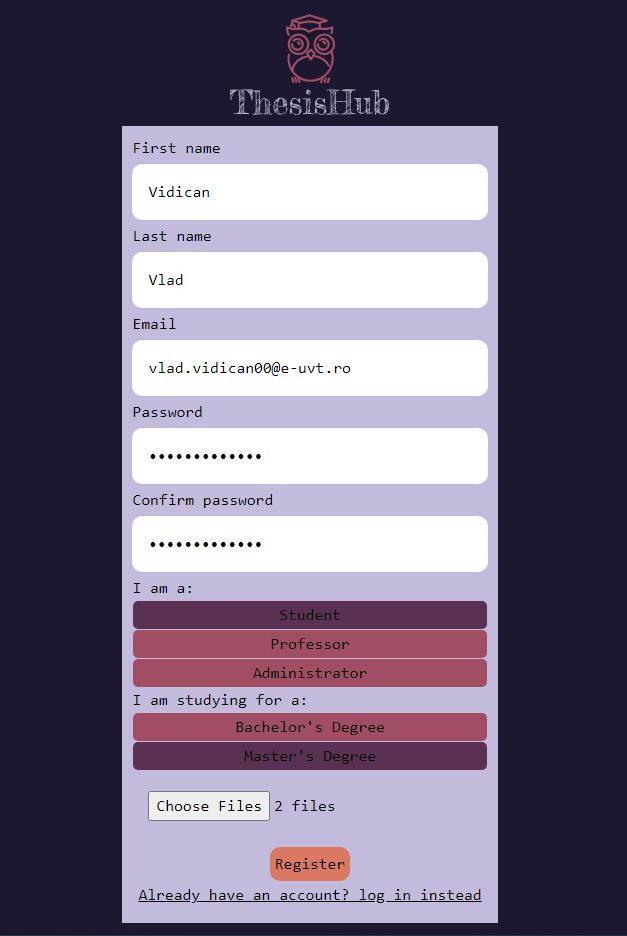
\includegraphics[scale=0.5]{images/RegisterForm.png}
    \caption{formular de înregistrare}
\end{figure}

Apoi utilizatorul va primi un cod de securitate pe adresa de email  folosită la crearea contului, pe care va trebui să îl introducă
in interfața deschisă după trimiterea cererii, această interfață îi permite de asemenea utilizatorului să solicite un cod nou de securitate
în cazul în care mail-ul inițial nu a fost livrat.
\begin{figure}[H]
    \centering
    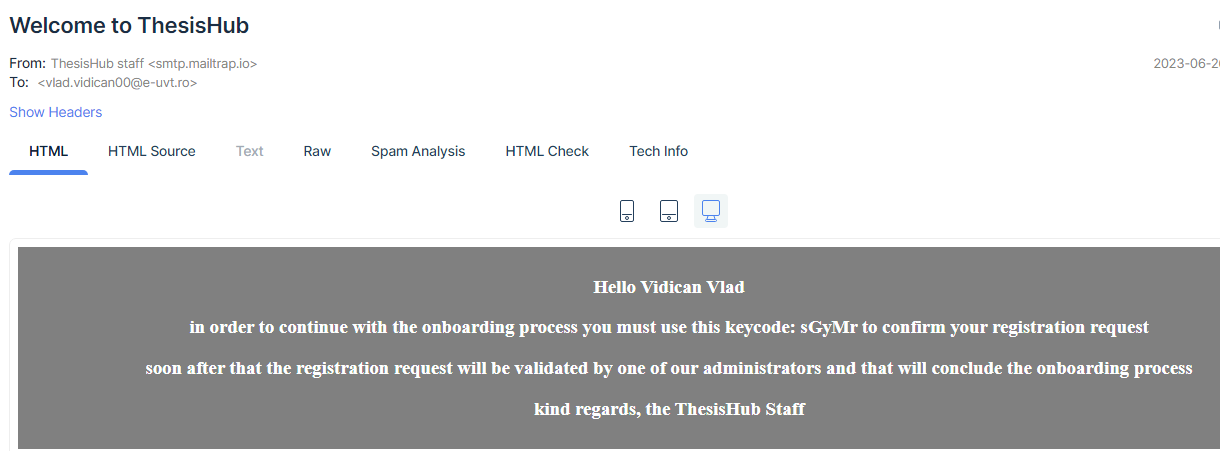
\includegraphics[scale=0.5]{images/RegisterEmail.png}
    \caption{exemplu email primit la înregistrare}
\end{figure}
\begin{figure}[H]
    \centering
    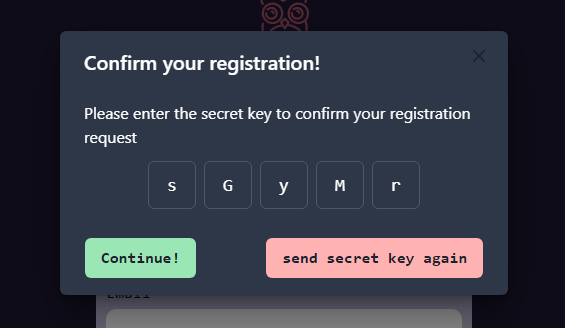
\includegraphics[scale=0.5]{images/SecurityKey.png}
    \caption{interfata pentru întroducerea codului de securitate}
\end{figure}

după ce utilizatorul introduce codul secret cererea lui de înregistrare este confirmată, 
ceea ce înseamnă că aceasta va fi acum vizibilă în bordul de gestionare a administratorilor (admin dashboard)
și urmează să fie revizuită de către unul din administratorii platformei, pentru acest pas utilizatorul nu are nimic de făcut,
odată ce cererea îi va fi aprobată acesta se va putea autentifica pe platformă, urmând să primească de asemenea un email de informare în legătură cu acest eveniment.
\begin{figure}[H]
    \centering
    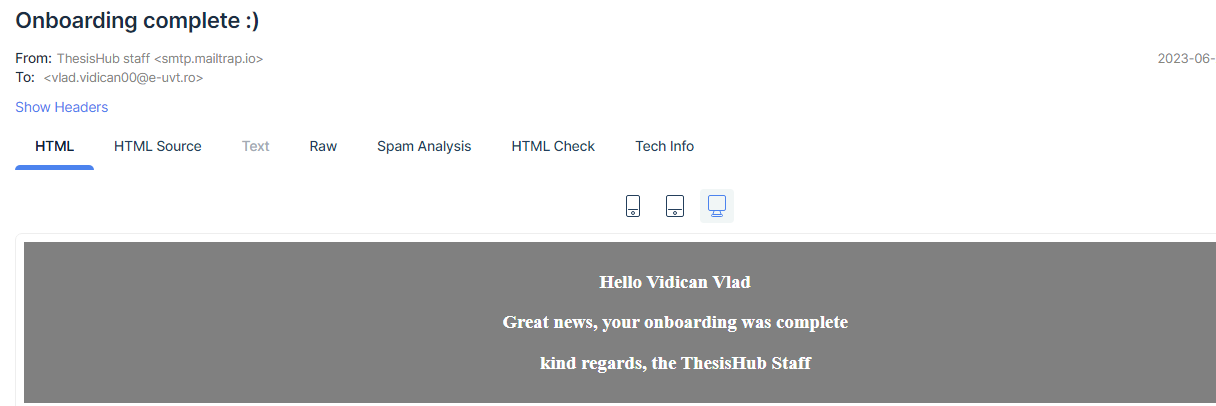
\includegraphics[scale=0.5]{images/OnboardingComplete.PNG}
    \caption{exemplu email de înformare}
\end{figure}
\begin{figure}[H]
    \centering
    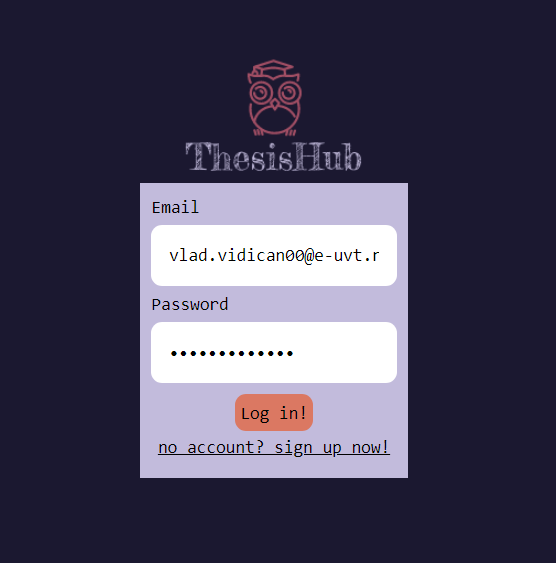
\includegraphics[scale=0.5]{images/LoginForm.PNG}
    \caption{Interfata autentificare}
\end{figure}
După o autentificare reușită, utilizatorul este redirectat către pagina principală, 
de aici utilizatorul poate să navigheze printre propunerile active de pe platformă.
Din motive de performanță am decis să implementez paginare pentru căutarea de propuneri,
serverul este configurat să returneze 4 elemente per pagină, în cazul în care nu toate propunerile sunt vizibile 
lista de propuneri permite scrolling, în partea de jos a pagini se află interfața pentru navigarea printre paginile de propuneri. 

Utilizatorul are opțiunea de a merge la pagina precedentă, pagina următoare sau la oricare dintre cele vizibile, apăsând 
pe unul dintre propuneri utilizator va fi redirecționat către pagina acelei propuneri
\begin{figure}[H]
    \centering
    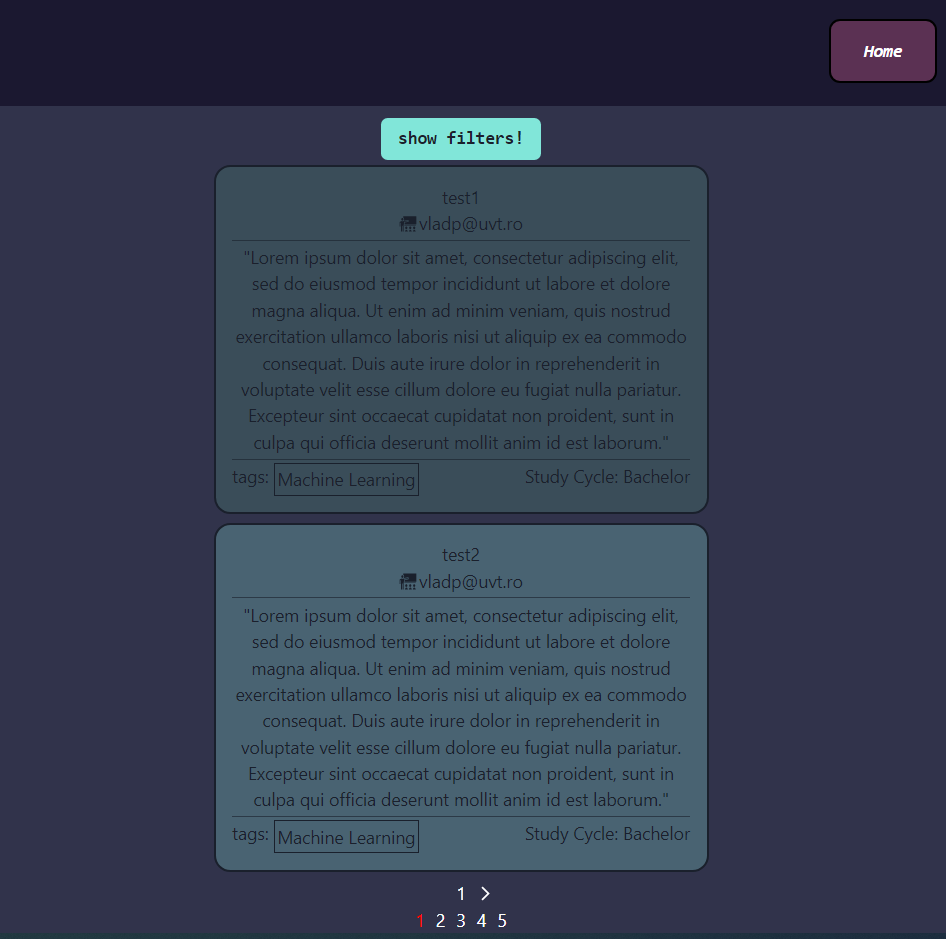
\includegraphics[scale=0.5]{images/HomePage.PNG}
    \caption{sistemul de navigare între propuneri din pagina principala}
\end{figure}
Platforma suportă și căutarea filtrată după propuneri, apăsând pe show filters utilizatorul poate să filtreze propunerile 
în funcție de următorii factori:
\begin{itemize}
    \item ciclu de studii pentru care este destinată propunerea.
    \item ce tip de cont a creat propunerea(student sau profesor).
    \item anumite cuvinte cheie din titlul propunerii.
    \item anumite cuvinte cheie din descrierea propunerii.
    \item etichetele în care se încadrează propunerile.
    aici utilizatorul poate să aleagă și care să fie relația între etichetele alese (să conțină cel puțin una sau pe toate)
    dacă sunt mai multe.
\end{itemize}
    după ce utilizatorul alege toate filtrele de care este interesat poate apăsa pe "Apply filters" pentru a reîmprospăta pagina
    doar cu propunerile ce respectă noile filtre, sau poate să apese la orice moment pe "reset filters" pentru a debifa toate filtrele adăugate
\begin{figure}[H]
    \centering
    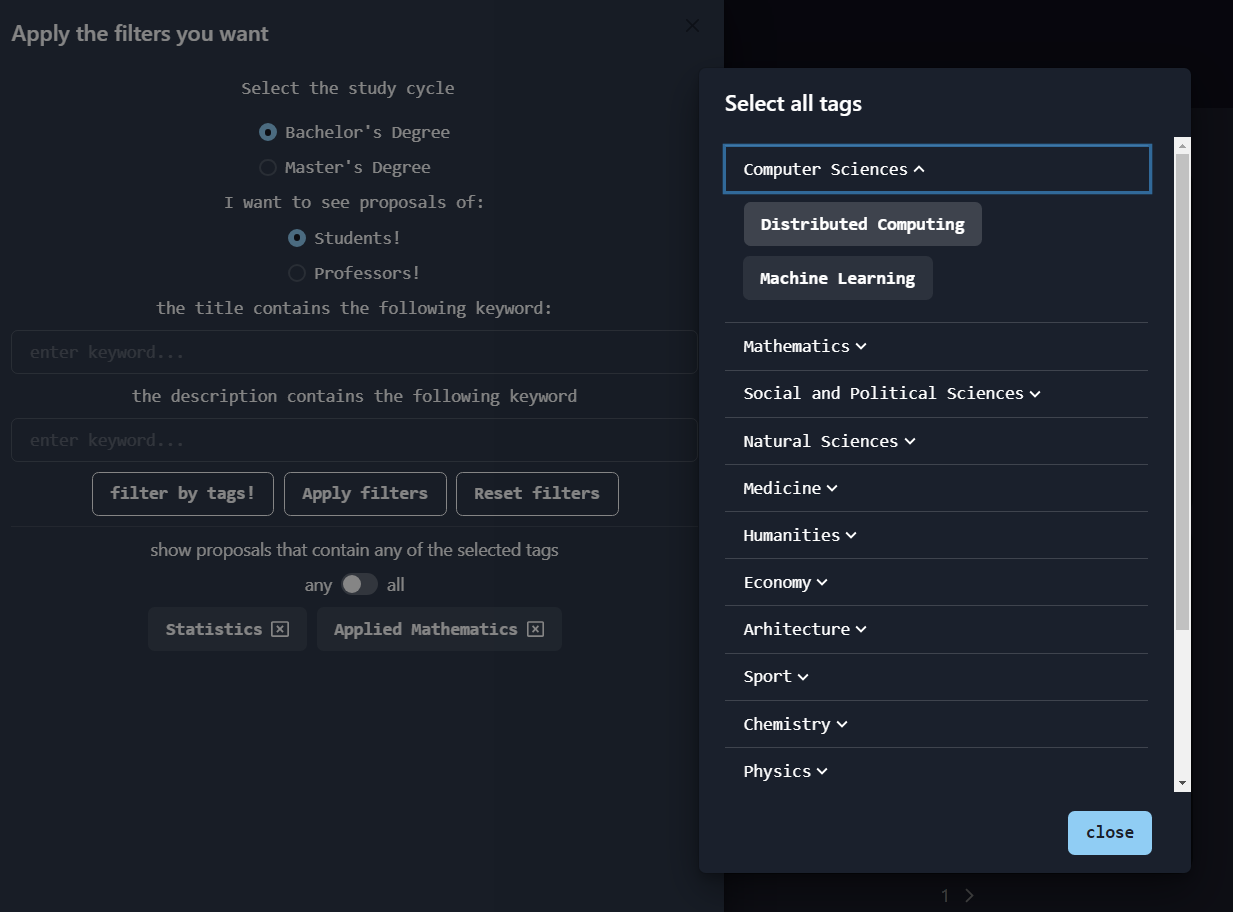
\includegraphics[scale=0.5]{images/advancedSearch.PNG}
    \caption{sistemul de cautare avanssata}
\end{figure}
Apăsând pe una dintre propuneri, utilizatorul va fi dus către pagina ei, aici are acces la mai multe informații despre această propunere, cum ar fi:
\begin{itemize}
    \item Lista de Atasamente.
    \item Lista de comentarii.
    \item Aplicatiile curente pe această temă.
\end{itemize}
și de aici acesta poate să:
\begin{itemize}
    \item Adauge un comentariu nou.
    \item să aplice pentru această propunere.
    \item să accepte una dintre aplicații dacă este deținătorul propunerii.
\end{itemize}
\begin{figure}[H]
    \centering
    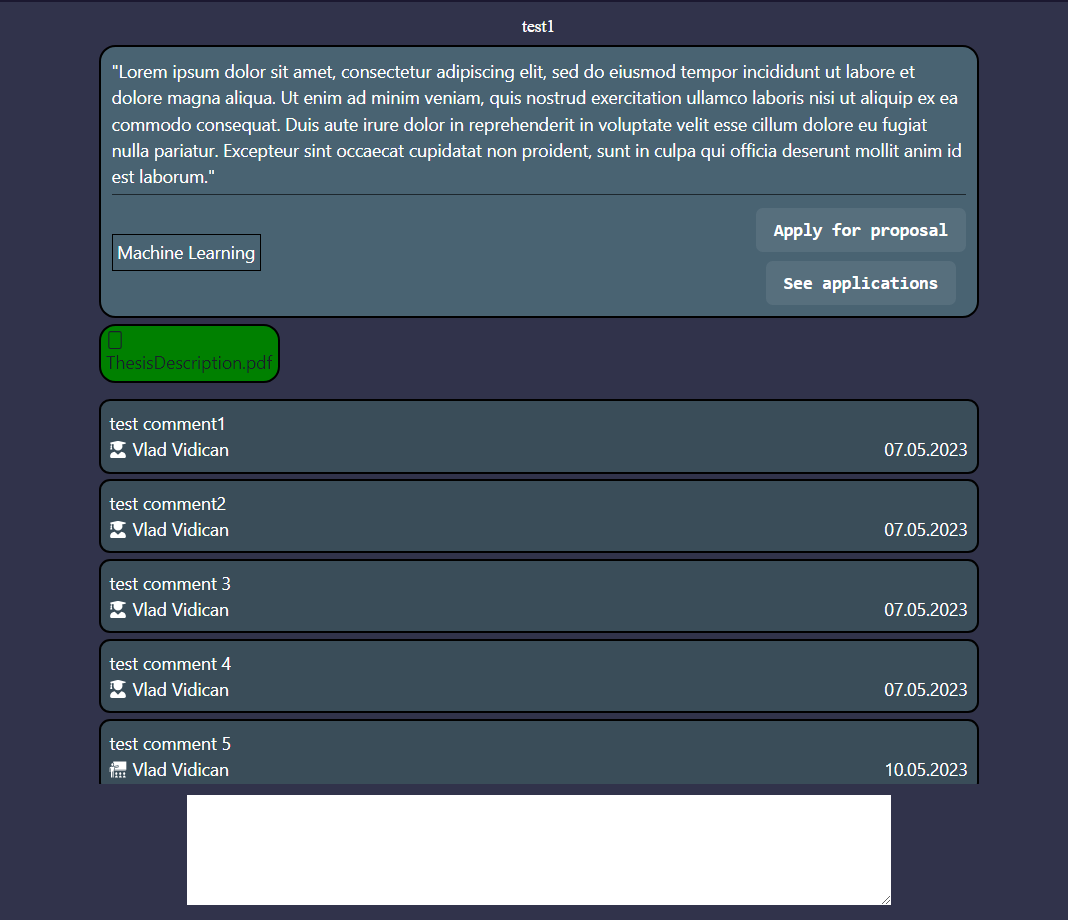
\includegraphics[scale=0.4]{images/ProposalPage.PNG}
    \caption{pagina de cautare google}
\end{figure}
\begin{figure}[H]
    \centering
    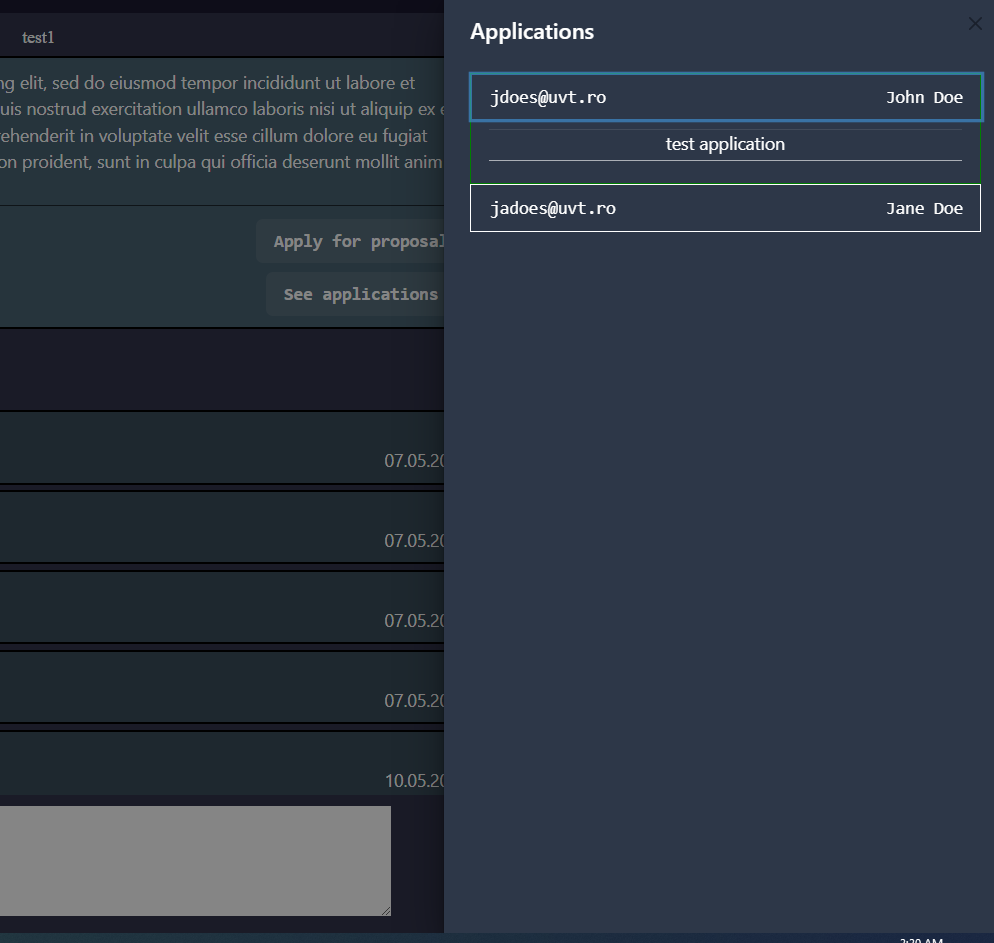
\includegraphics[scale=0.4]{images/Application.PNG}
    \caption{exemplu lista de aplicații a unei propuneri}
\end{figure}
Utilizatorul poate să își creeze propria lui propunere apăsând butonul "Create proposal" din bara de navigare
mai apoi acesta trebuie să completeze următoarele câmpuri:
\begin{itemize}
    \item Titlul propunerii.
    \item Descrierea propunerii
    \item Atașamente (opțional)
    \item să aleagă cel puțin o eticheta din cele disponibile
\end{itemize}
pentru a atașa etichete propunerii utilizatorul trebuie să aleagă mai întâi o categorie din bara din dreapta a pagini 
și din categoria aleasă poate să asocieze etichetele disponibile, utilizatorul nu este însă limitat la o singură categorie
\begin{figure}[H]
    \centering
    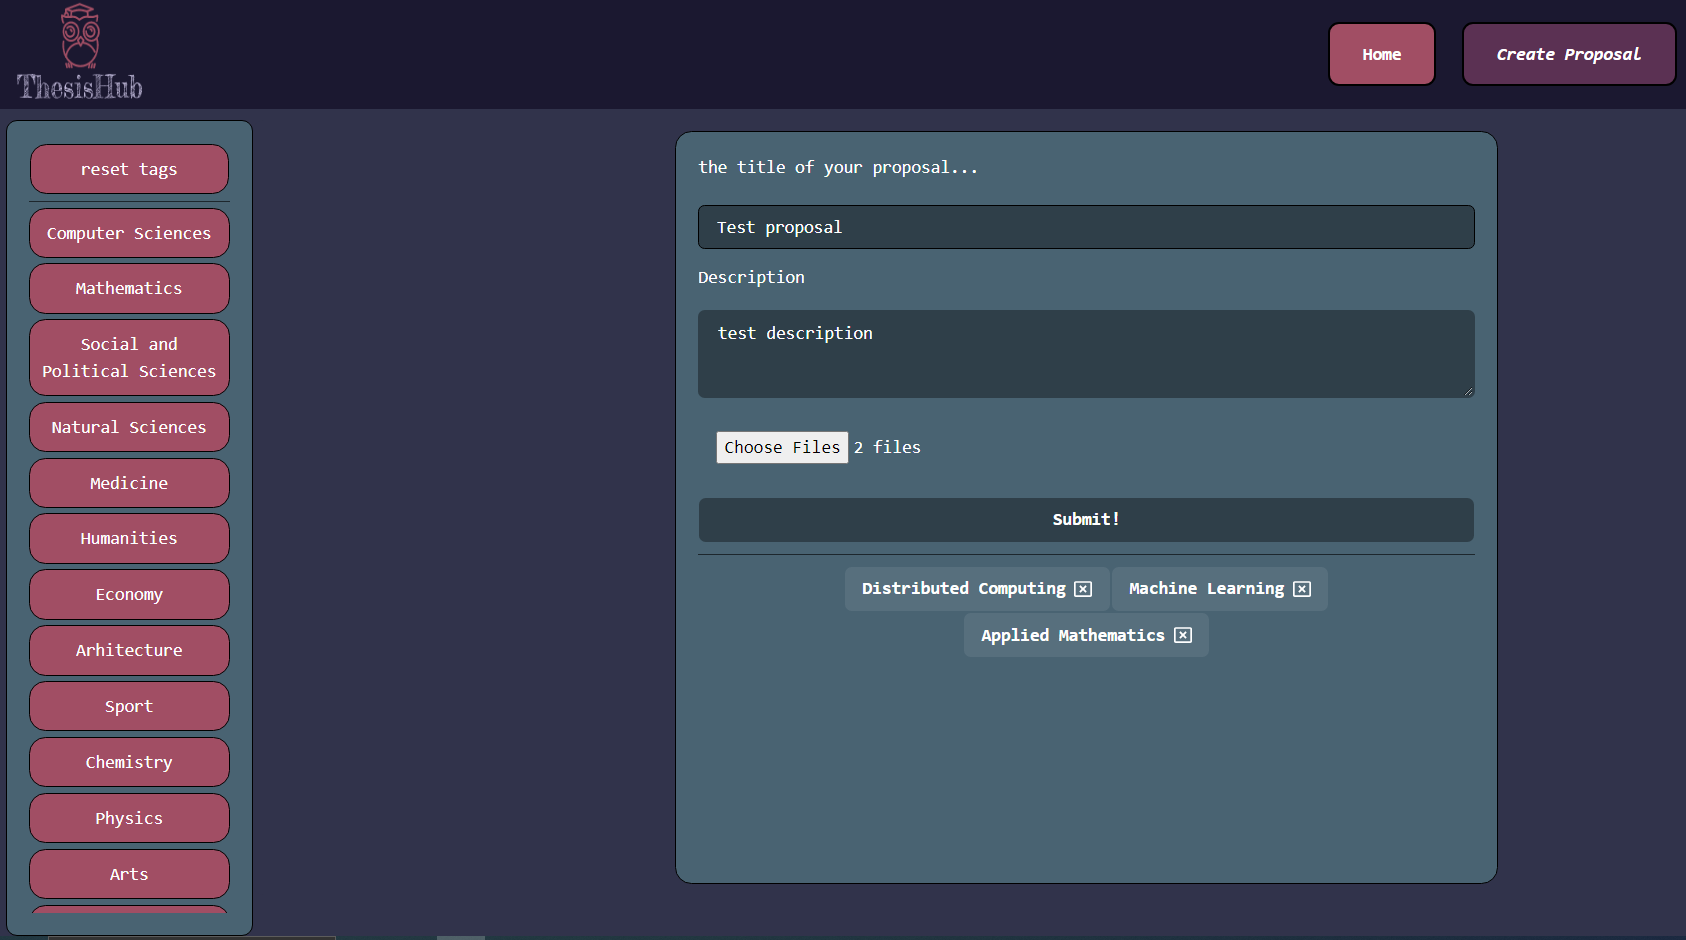
\includegraphics[scale=0.4]{images/CreateProposalPage.PNG}
    \caption{pagina pentru crearea propunerilor noi}
\end{figure}
\begin{figure}[H]
    \centering
    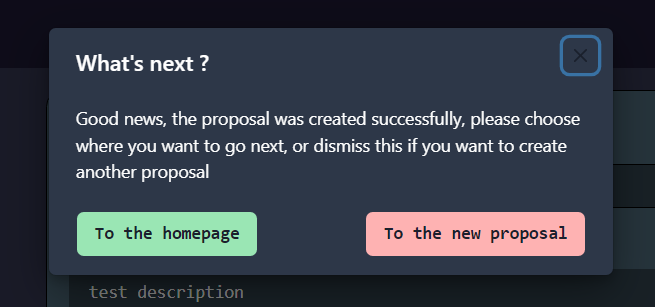
\includegraphics[scale=0.7]{images/ProposalCreated.PNG}
    \caption{Propunere creata cu success}
\end{figure}
Pentru a putea accesa pagina de mesagerie utilizatorul trebuie să apese butonul "Conversations" din bara de navigare.

Odată ajuns pe pagina de mesagerie utilizatorul poate să aleagă una dintre conversațiile actuale
Apăsând pe aceasta din bara laterală, sau poate să apese "Add Users" pentru a iniția conversații noi.
Dacă utilizatorul dorește să inițieze conversații noi acesta trebuie doar să introducă adresa de email
a acelei persoane în câmpul pentru căutarea utilizatorilor, însă acest lucru nu este necesar
ca utilizatorii să cunoască adresa de email în totalitate a persoanelor cu care doresc să inițieze o conversație, 
sistemul oferind sugestii în funcție de literele introduse.

\begin{figure}[H]
    \centering
    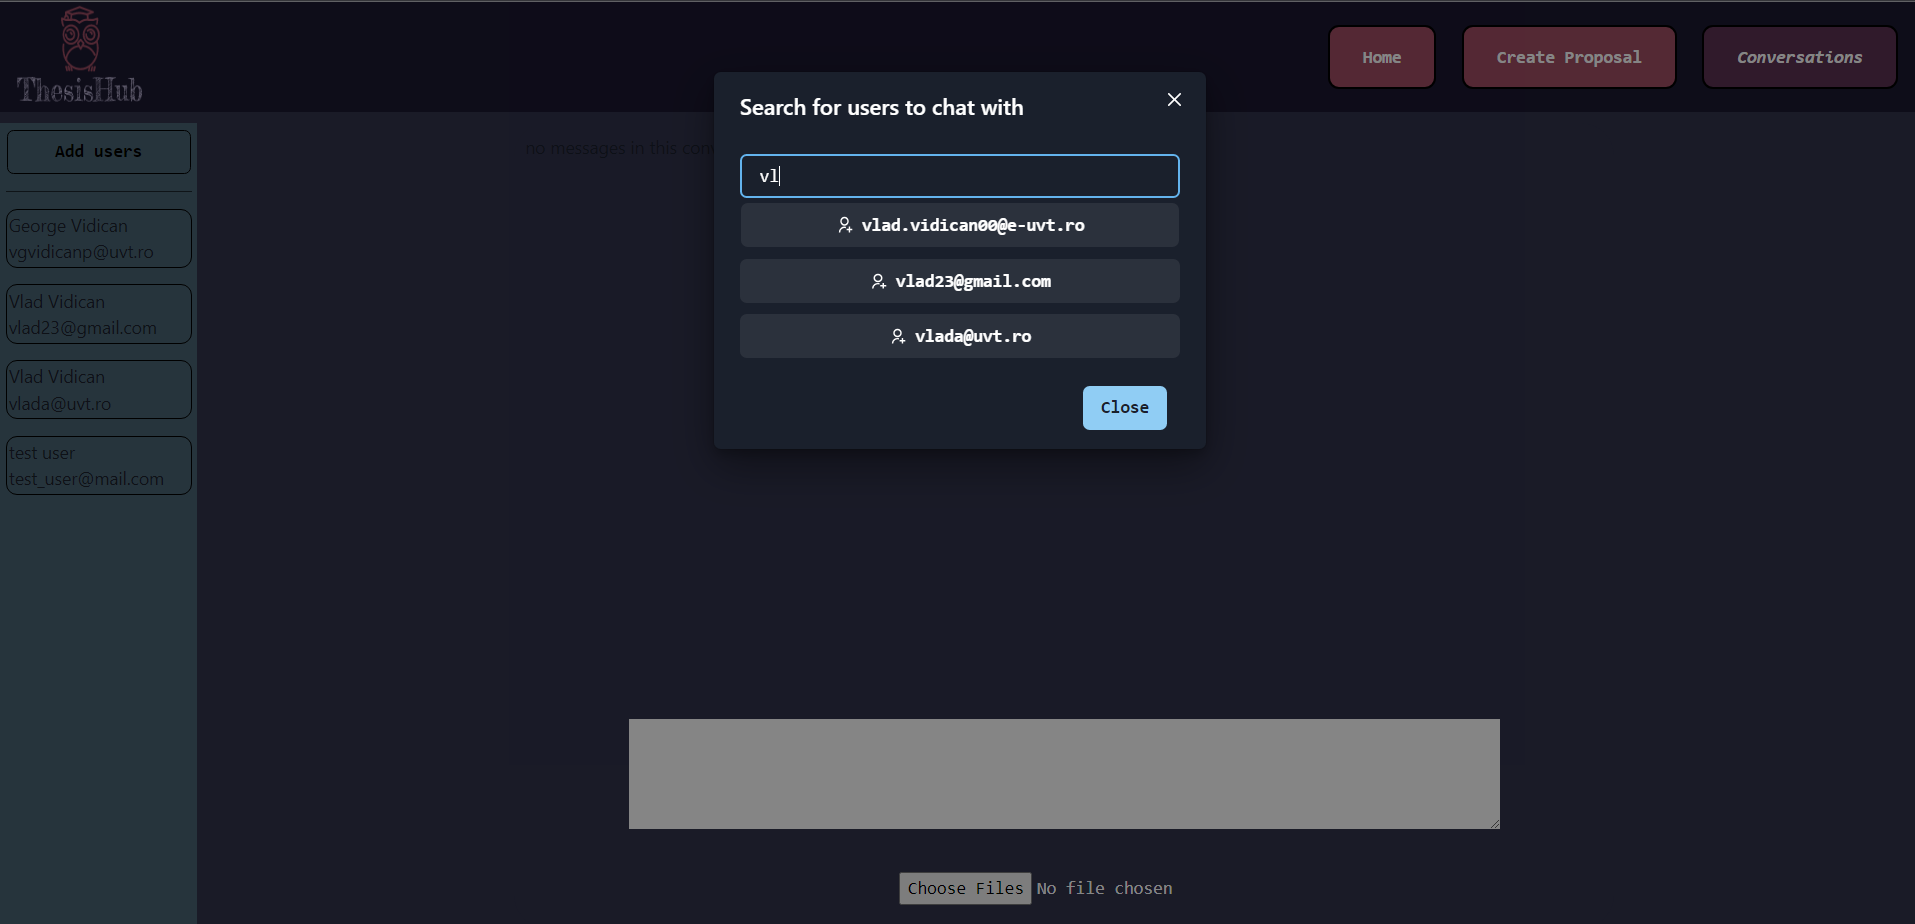
\includegraphics[scale=0.3]{images/AddUser.PNG}
    \caption{Interfata de înitiere a unei conversatie}
\end{figure}
Odată cu alegerea unei conversații utilizatorii pot trimite mesaje, acest lucru se poate face  
introducând textul dorit în zona de mesaje și apăsând tasta ENTER,  
sistemul suportă și mesaje ce se întind pe mai multe linii, utilizatorul poate să înceapă o linie nouă apăsând tastele SHIFT + ENTER
. Sistemul suportă de asemenea și trimiterea de fișiere, acestea sunt legate de mesaje, utilizatorul trebuie astfel doar să aleagă
fișierele dorite și acestea vor fi trimise automat cu următorul mesaj.
\begin{figure}[H]
    \centering
    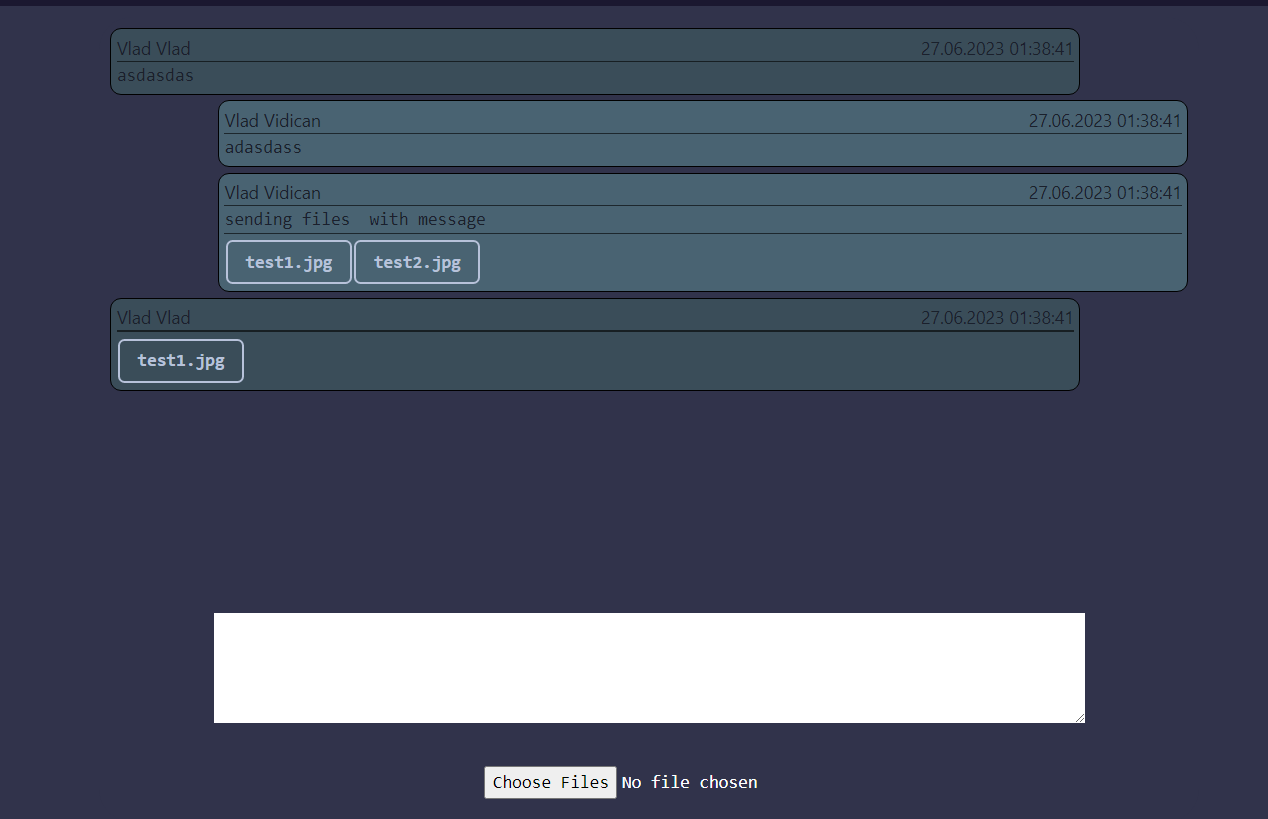
\includegraphics[scale=0.3]{images/SendMessages.PNG}
    \caption{Interfata Mesagerie}
\end{figure}
Administratorii au de asemenea posibilitatea de a accesa bordul de gestiune din bara de navigare(dashboard), 
aici pot vedea toate cererile de înregistrare active de pe platforma, pe lângă datele contului 
administratorii pot și să revizuie dovezile de identitate atașate cererilor de înregistrare,
în cazul în care administratorul decide să respingă o cerere atunci acesta este nevoit să îi ofere utilizatorului și o justificare 
pentru decizia luată, un email de informare fiind trimis utilizatorului ulterior.
\begin{figure}[H]
    \centering
    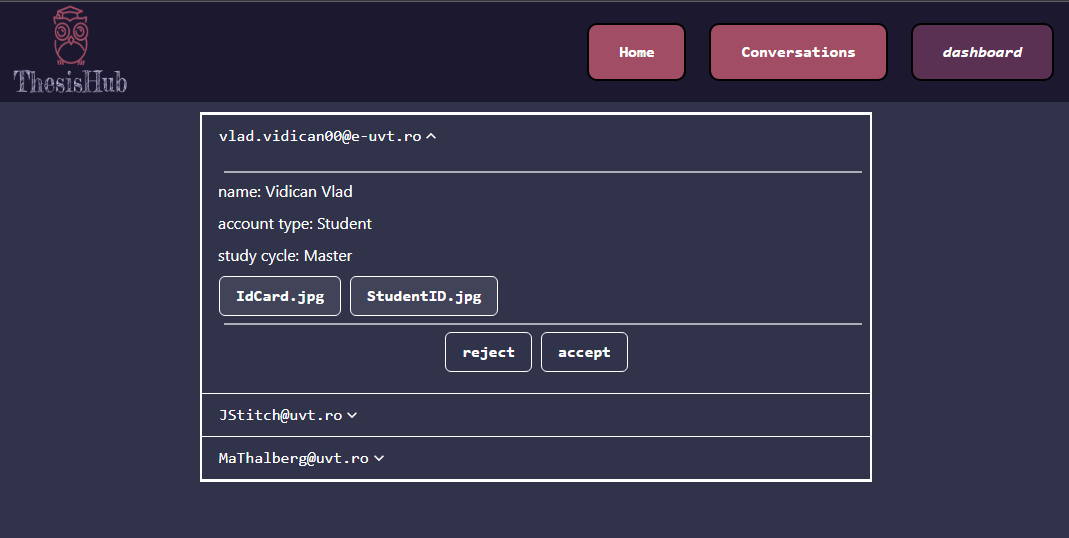
\includegraphics[scale=0.5]{images/Dashboard.PNG}
    \caption{Bordul de gestiune a administratorilor}
\end{figure}
\begin{figure}[H]
    \centering
    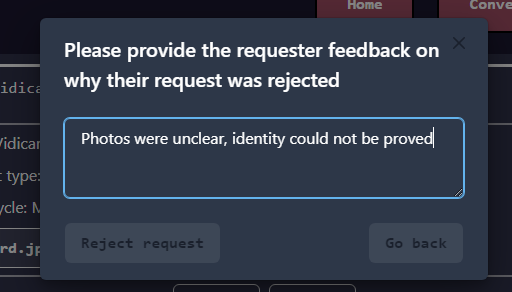
\includegraphics[scale=0.7]{images/RejectRequest.PNG}
    \caption{Exemplu respingere cerere de înregistrare}
\end{figure}
\chapter{Concluzii și direcții viitoare}
\section{direcții viitoare}
Deși aplicația în starea ei actuală oferă funcționalitățile propuse aceasta are încă 
potențial de dezvoltare, spre exemplu trecerea spre un sistem care să suporte mai multe universități. 
Deși în momentul de față accesul nu este restricționat explicit unei singure instituții
sistemul nu suportă în starea sa actuală separarea logică a entităților în funcție de universitatea de apartenență.
Această funcționalitate este însă necesară pentru a putea fi extinsă, fără aceasta administratorii unei universități ar avea drepturi elevate
în ceea ce privește gestionarea utilizatorilor asupra tuturor celorlalte universități integrate în sistem.

Pentru a obține acest rezultat un prim plan ar fi adăugarea unei colecții de universități și modificarea schemei colecțiilor: 
user, userTemp și proposal pentru a avea și o referință către o universitate, ar mai fi de asemenea nevoie de trecerea la un sistem
cu două tipuri de administratori:
\begin{itemize}
    \item Administratori locali: aceștia vor avea dreptul de a gestiona utilizatorii din aceeași universitate ca și ei înșiși
    \item Administratori ai aplicației: aceștia nu aparțin unei universități anume și vor fi responsabili de adăugarea de 
    universități, categorii și etichete noi în sistem, aceștia nu se vor ocupa de gestionarea utilizatorilor în general excepții fiind 
    adăugarea administratorului inițial al unei universități și adăugarea altor administratori de acest tip
\end{itemize}

O altă oportunitate de dezvoltare ar fi implementarea unei aplicații mobile, dat fiind faptul ca serverul de backend 
este separat de logica generării de pagini html și livrării de conținut static acesta ar putea fi integrat cu un client
de tip mobil fără a necesita nici o schimbare.

Posibilitatea de a folosi react native pentru dezvoltarea aplicației mobile este de asemenea un factor important deoarece
ar rezulta într-o portare mai ușoara, Deși codul nu poate fi mapat unu la unu între react și react native, aceste tehnologii folosind 
în spate elemente primitive diferite, acestea au însă un grad de similitudine ridicat
\section{Concluzii}
Această lucrare de licență a avut ca scop dezvoltarea unei posibile soluții pentru una dintre problemele 
întâmpinate de catre studenți, mai exact lispa unui proces bine stabilit si convenient 
în ceea ce privește găsirea unui coordonator. Deși universitațile au de regula un proces bine definit 
cu precădere la evoluția si asistarea studentului in privința realizării lucrării, acest proces lipsește in ceea ce privește 
potrivirea studenților cu profesorii coordonatori de regulă fiind asumată mai degrabă o abordare "ad-hoc".
Acest Pas ar putea fi insă considerat unul dintre cei mai importanți, deoarece atât compatibilitatea student-profesor căt și interesul real al 
studentului fața de tema lucrârii sunt esențiale pentru o lucrare reușită.

Aplicația in starea ei actuală ofera urmatoarele facilitați:
\begin{itemize}
    \item Posibilitatea de a posta sau aplica la teme de licența/master.
    \item Căutare avansată care permite un nivel de specificitate ridicat cu scopul de a usura găsirea temelor de interes.
    \item Un mediu prielnic pentru comunicarea dintre student si profesor.
    \item Un proces robust de validare a identității care să permită restrictionarea accesului la platforma doar persoanelor vizate.
\end{itemize}
Datorită celor enumerate mai sus, consider ca lucrarea a rezultat cel puțin într-un prototip bun cu potențial de dezvoltare spre o soluție la problema prezentată anterior
\begin{thebibliography} {10}
    \bibitem{1}
    Banks, A., Parcello, E. [2017]. Learning React. Functional web development with react and redux. USA: O’Reilly Media, Inc. 
    \bibitem{2}
    Hahn, Evan M. [2016]. Express in Action. Writing, building and testing Node.js applications. New York: Manning Publications Co.
    \bibitem{3}
    Young, A. et al. [2017] Node.js in action second edition. New York: Manning Publications. 
    \bibitem{4}
    Banker, K. et al. [2016] MongoDB in action second edition. New York: Manning Publications. New Tork: Manning Publications. 
    \bibitem{5}
    Flanagan D. [2011] Javascript: the definitive guide sixth edition. USA: O’Reilly Media, Inc.
    
    \end{thebibliography}
\end{document}
